\documentclass[openany, oneside]{book}
%Packages Used-----------------------------------------------------
\usepackage{color}
\usepackage{hyperref}
\usepackage{amsmath}
\usepackage{amsfonts}
\usepackage{amssymb}
\usepackage{tabto}
\usepackage[utf8]{inputenc}

\usepackage{booktabs}


\usepackage{nameref}

\usepackage{geometry}
\geometry{
	b5paper,
	hmargin=20mm,
	vmargin=15mm,
	includehead,
	includefoot,
%	showframe
}

\usepackage{tikz}
\usetikzlibrary{
	shapes.geometric,
	arrows,
}
\usepackage{pgfplots}
\pgfplotsset{compat=1.18}

\usepackage{graphicx}
\usepackage{siunitx}

%End of Packages Used----------------------------------------------
\title{Mathematical Formulae\\\begin{large}
A Book of High School and Engineering Common Core Mathematical Formulae
\end{large}}
\date{December, 2020}
\author{Agnij Mallick}


\hypersetup{
    colorlinks=true,
    linkcolor=black,
    urlcolor=black,
    linktoc=all
}


\pagestyle{myheadings}
\markright{}

\begin{document}
\frontmatter
\maketitle

\tableofcontents
\newpage

\mainmatter

\part{Algebra}
\chapter{Logarithm}
\section{Basic Formulae}
% Refactor completely. Add sections:
% Domain of definition
% Arithmetic Properties
For $a^x=b$:
\begin{align}
	\log_a x \text{, for all }x\leq0\text{ is undefined}\\
	\log_a b=x\text{, }bax\neq1\text{, }a\neq1\\
	\log_b a^m=m\log_b a\text{, for } a^m=b\\
	a^{\log_a x}=x\\
	a^{\log_b c}=c^{\log_b a}\\
	\frac{1}{\log_a b}=\log_b a\\
	\log_c (ab)=\log_c a+\log_c b\\
	\log_c (\frac{a}{b})=\log_c a-\log_c b\\
	\abs{\log_a x} =
	\begin{cases}
		-\log_a x, \text{ if } \, 0 < x < 1\\
		\log_a x, \text{ if } \, 1\leq x < \infty \\
	\end{cases}
\end{align}


\section{Series}
\begin{align}
	e^x
		&= 1 + \frac{x}{1!} + \frac{x^2}{2!} + \frac{x^3}{3!} + \ldots
		= \sum_{i=0}^{\infty} \frac{x^i}{i!}\\
	\log(1+x)
		&= x - \frac{x^2}{2} + \frac{x^3}{3} - \frac{x^4}{4} + \ldots
		= \sum_{i=1}^{\infty} (-1)^{(i-1)} \frac{x^i}{i}
\end{align}

\chapter{Complex Number}
\section{Basic Formulae}
For $z=x+iy$,
\begin{align}
	&\abs{z} = \sqrt{x^2+y^2}\\
	&\tan \theta = \frac{y}{x}\\
	&\bar{z} = x - iy
\end{align}


\section{Arithmetic Operation of Complex Number}
For two complex numbers $z_1=x_1+iy_1$ and $z_2=x_2+iy_2$:
\begin{align}
	&z_1+z_2=(x_1+x_2)+i(y_1+y_2)\\
	&z_1 \cdot z_2=(x_1x_2-y_1y_2)+i(x_1y_2+x_2y_1)\\
	&\abs{z_1\cdot z_2} = \abs{z_1} \cdot \abs{z_2}\\
	&\frac{z_1}{z_2}=\frac{(x_1x_2+y_1y_2)+i(x_2y_1-x_1y_2)}{{a_2}^2+{b_2}^2}\\
	&\abs*{\frac{z_1}{z_2}} = \frac{\abs{z_1}}{\abs{z_2}}
\end{align}


\section{Euler's Formula}
\begin{equation}
	z=re^{i\theta}\text{, where $r= \abs{z}$, $e^{i\theta}=\cos \theta + i \sin \theta$, and $\theta=\tan^{-1}\frac{y}{x}$}
\end{equation}


\section{Trigonometric Ratios in Complex Form}
\begin{align}
	e^{i\theta}+e^{-i\theta} &= 2\cos\theta\\
	\implies \cos \theta &= \frac{e^{i\theta}+e^{-i\theta}}{2}
\end{align}
\begin{align}
	e^{i\theta}-e^{-i\theta} &= 2\sin\theta\\
	\implies \sin \theta &= \frac{e^{i\theta}-e^{-i\theta}}{2}
\end{align}


\section{De Moivre's Formula}
\begin{equation}
	(\cos\theta + i\sin\theta)^n = \cos(n\theta) + i\sin(n\theta)
\end{equation}


\section{Application of Euler's and De Moivre's Formula}
For $z_1 = r_1 e^{i\theta_1}$ and $z_2 = r_2 e^{i\theta_2}$
\begin{align}
	&z_1\cdot z_2 = r_1r_2 e^{i(\theta_1+\theta_2)}\\
	&\frac{z_1}{z_2}=\frac{r_1}{r_2}e^{i(\theta_1-\theta_2)}
\end{align}


\section{Roots of Unity}
\begin{equation}
	\sqrt[n]{1}=e^{i\frac{2k\pi}{n}},\text{ where } k \in [0,n-1]
\end{equation}


\section{Important Relations of Complex Numbers}
\begin{align}
	\abs{z_1+z_2} \leq \abs{z_1} +\abs{z_2}\\
	\abs{z_1-z_2} \leq  \abs{z_1} + \abs{z_2}\\
	\abs{z_1-z_2} \geq  \abs{z_1} - \abs{z_2}\\
	\abs{z_1+z_2} \geq \abs{\abs{z_1} - \abs{z_2}}\\
	\abs{z_1+z_2}^2 = 2(\abs{z_1}^2 + \abs{z_2}^2) % WTF? CHECK
\end{align}

\chapter{Progression}
\section{Arithmetic Progression (A.P.)}
An arithmetic sequence is $a,a+n,a+2n,...\infty$ or $t_n=a+(n-1)d$, where $a$ is the first term, $d$ is the common difference, and $n$ is the $n^{th}$-term.

An arithmetic series is $a+(a+d)+(a+2d)+...\infty$.

\subsection{Sum of A.P. Series}
\begin{align}
	S_n=a+(a+d)+...+(a+\overline{n-2}d)+(a+\overline{n-1}d)\nonumber\\
	S_n=(a+\overline{n-1}d)+(a+\overline{n-2}d+...+(a+d)+ a\nonumber\\
	\Rightarrow 2S_n=n(2a+\overline{n-1}d)\nonumber\\
	\Rightarrow S_n=\dfrac{n}{2}(2a+\overline{n-1}d)
\end{align}

\subsection{Important Relation}
If the three terms $a,b,c$ are in A.P., then
\begin{align}
	2b=a+c
\end{align}


\section{Geometric Progression (G.P.)}
An geometric sequence is $a,ar,ar^2,...\infty$ or $t_n=ar^{n-1}$, where $a$ is the first term, $r$ is the common ratio, and $n$ is the $n^{th}$-term.

An geometric series is $a+ar+ar^2+...\infty$.

\subsection{The Value of 'r'}
\begin{align}
	r=\frac{t_2}{t_1}=\frac{t_3}{t_2}=...=\frac{t_{n}}{t_{n-1}}
\end{align}

\subsection{Sum of a G.P.  Series}
For a definite G.P. series, where there are $n$ terms in the series, the sum of the series is:
\begin{align}
	S_n=\dfrac{a\lvert r^n-1 \rvert}{\lvert r-1 \rvert}
\end{align}

For an infite G.P. series the sum of the series is defined for $r<1$. Sum of such a series is:
\begin{align}
	S_\infty=\dfrac{a}{1-r}
\end{align}

\subsection{Important relations}
If the three terms $a,b,c$ are in G.P., then:
\begin{align}
	b^2=ac
\end{align}


\section{Harmonic Progression (H.P.)}
If $a,b,c$ are terms of an H.P. then $\frac{1}{a},\frac{1}{b},\frac{1}{c}$ are in A.P.
\begin{align}
	\therefore \dfrac{2}{b}=\dfrac{1}{a}+\dfrac{1}{c}\\
	\Rightarrow b=\dfrac{2ac}{a+c}
\end{align}


\section{\large{Arithmetico-Geometric Progression (A.G.P.)}}
Sequence $a, (a+d)r, (a+2d)r^2,...,(a+\overline{n-1}d)r^{n-1}$, where $a\rightarrow$first term of A.G.P., $d\rightarrow$common difference, and $r\rightarrow$common ratio.

\subsection{Sum of A.G.P.:}
For an infinite A.G.P. series, the sum is defined for $r<1$:
\begin{align}
	S_\infty=\dfrac{a}{1-r}+\dfrac{dr}{(1-r)^2}
\end{align}


\section{Special Series}
For $n\in\mathbb{N}$
\begin{align}
	1+2+3+....+(n-1)+n=\dfrac{n(n-1)}{2}\\
	1^2+2^2+3^2+...+(n-1)^2+n^2=\dfrac{n(n+1)(2n+1)}{6}\\
	1^3+2^3+3^3+...+(n-1)^3+n^3=[\dfrac{n(n-1)}{2}]^2
\end{align}

\subsection{Riemann Zeta Function}
\begin{equation}
	\zeta(s)=\sum_{n=1}^\infty \dfrac{1}{n^s}
\end{equation}

\subsection{Riemann's Infinite Series as an Integration}
\label{riemannsum}
\begin{align}
	\lim_{n\to\infty} \dfrac{1}{n}\sum_{i=r_1}^{r_2} f(\frac{i}{n})=\int_{\frac{r_1}{n}}^{\frac{r_2}{n}} f(x) dx
\end{align}

\large{\chapter{Test of Convergence of Infinite Series}}
If $a_1,a_2,a_3,...,a_n$ is a sequence by $a_n$ and their sum of series is $S_n$, then the following apply.
\section{Definition}
If \begin{equation}\lim_{n\to\infty} S_n=l\nonumber\end{equation} where $l$ is a finite value, the series $S_n$ is said to converge. A non-convergent series is called a divergent series.
\section{Tests of Convergence}
\subsection{Comparison Test}
If $u_n$ and $v_n$ are two positive series, then:
\begin{enumerate}
	\item \begin{enumerate}
		\item $v_n$ converges
		\item $u_n\leq v_n \forall n$
		Then $u_n$ converges.
	\end{enumerate}
	\item \begin{enumerate}
		\item $v_n$ diverges
		\item $u_n\geq v_n \forall n$
		Then $u_n$ diverges.
	\end{enumerate}
\end{enumerate}

\subsection{Limit Form}
If \begin{equation}\lim_{x\to\infty} \dfrac{u_n}{v_n} = l \nonumber\end{equation} where $l$ is a finite quantity $\neq0$, then $u_n$ and $v_n$ converge and diverge together.

\subsection{Integral Test or Maclaurin-Cauchy Test}
For a series
\begin{equation}
	\sum_{i=N}^{\infty} f(x)\text{, where } N\in\mathbb{Z}
\end{equation}
will only converge if the improper integral
\begin{equation}
	\int_{N}^{\infty} f(x) dx
\end{equation}
is finite.
\paragraph{}
If the improper integral is finite, the upper and lower limit of the infinite series is given by:
\begin{equation}
	\int_{N}^{\infty} f(x) dx \leq \sum_{i=N}^{\infty} f(x) \leq f(N)+\int_{N}^{\infty} f(x) dx
\end{equation}
\subsection{Ratio Test}
If, for two series $\sum u_n$ and $\sum v_n$:

\begin{enumerate}
	\item \begin{enumerate}
		\item $\sum v_n$ converges
		\item from or after a particular term $\dfrac{u_n}{u_{n+1}}>\dfrac{v_n}{v_{n+1}}$, then $u_n$ converges.
	\end{enumerate}
	\item \begin{enumerate}
		\item $\sum v_n$ diverges
		\item from or after a particular term $\dfrac{u_n}{u_{n+1}}<\dfrac{v_n}{v_{n+1}}$, then $u_n$ diverges.
	\end{enumerate}
\end{enumerate}

\subsection{D'Alembert's Ratio Test}
\begin{equation}
	\lim_{n\to\infty} \dfrac{u_n}{u_{n+1}}=\lambda
\end{equation}
\begin{itemize}
	\item series converges if $\lambda<1$
	\item series diverges if $\lambda>1$
	\item fails if $\lambda=1$
\end{itemize}

\subsection{Rabbe's Test}
\begin{equation}
	\lim_{n\to\infty} n[\dfrac{u_n}{u_{n+1}}-1]=\kappa
\end{equation}
\begin{itemize}
	\item series converges if $\kappa<1$
	\item series diverges if $\kappa>1$
	\item fails if $\kappa=1$
\end{itemize}

\subsection{Cauchy's Root Test}
\begin{equation}
	\lim_{n\to\infty} \lvert u_n \rvert=\lambda
\end{equation}
\begin{itemize}
	\item series converges for $\lambda<1$
	\item series diverges for $\lambda>1$
	\item test fails for $\lambda=1$
\end{itemize}

\subsection{Logarithmic Test}
\begin{equation}
	\lim_{n\to\infty} n\log(\dfrac{u_n}{u_{n+1}})=\kappa
\end{equation}
\begin{itemize}
	\item series converges for $\kappa<1$
	\item series diverges for $\kappa>1$
	\item test fails for $\kappa=1$
\end{itemize}
%End of Chapter-----------------------------------------------------------------------------------
\large{\chapter{Determinants}}
\section{Definition}
For a determinant:
\begin{equation}
	\Delta=\begin{vmatrix}
		a_1&b_1&c_1\\
		a_2&b_2&c_2\\
		a_3&b_3&c_3
	\end{vmatrix}=a_1\begin{vmatrix}b_2&c_2\\b_3&c_3\end{vmatrix}-b_1\begin{vmatrix}a_2&c_2\\a_3&c_3\end{vmatrix}+c_1\begin{vmatrix}a_2&b_2\\a_3&b_3\end{vmatrix}
\end{equation}
\subsection{Minor and Cofactor}
For a third order determinant
$\begin{vmatrix}
	a_1&b_1&c_1\\
	a_2&b_2&c_2\\
	a_3&b_3&c_3
\end{vmatrix}$, the minor of $a_{11}$ is $M_{11}=\begin{vmatrix}b_2&c_2\\b_3&c_3\end{vmatrix}$, i.e., all the terms of the determinant expect those in the same row and columns as the one of which the minor is being calculated.
\paragraph{}Cofactor $C_{ij}=(-1)^{i+j} M_{ij}$

\section{Important Properties}
\begin{enumerate}
	\item Transposing a determinant does not alter its value.
	\item If rows and columns are interchanges $m$ times, the value of the new determinant is
	\begin{equation}
		\Delta'=(-1)^m \Delta
	\end{equation}
	\item If two parallel lines are equal, then $\Delta=0$
	\item For $\Delta=\begin{vmatrix}a_1&b_1&c_1\\a_2&b_2&c_2\\a_3&b_3&c_3\end{vmatrix}$ and $\Delta_1=\begin{vmatrix}ka_1&kb_1&kc_1\\a_2&b_2&c_2\\a_3&b_3&c_3\end{vmatrix}$, then $\Delta_1=k\Delta$
	\item For $\Delta=\begin{vmatrix}a_1&b_1&c_1\\a_2&b_2&c_2\\a_3&b_3&c_3\end{vmatrix}$ and $\Delta_1=\begin{vmatrix}ka_1&b_1&c_1\\ka_2&b_2&c_2\\ka_3&b_3&c_3\end{vmatrix}$, then $\Delta_1=k\Delta$
	\item For $C_n\rightarrow k_1C_l+k_2C_m+k_3C_n$ or $R_n\rightarrow k_1R_l+k_2R_m+k_3R_n$, $\Delta'=\Delta$
\end{enumerate}

\section{Cramer's Rule}
For a system of equations:
\begin{align}
	a_1x+b_1y+c_1z=d_1\nonumber\\
	a_2x+b_2y+c_2z=d_2\nonumber\\
	a_3x+b_3y+c_3z=d_3\nonumber
\end{align}
the following determinants are defined:
\begin{align}
	D=\begin{vmatrix}a_1&b_1&c_1\\a_2&b_2&c_2\\a_3&b_3&c_3\end{vmatrix}\nonumber\\
	D_x=\begin{vmatrix}d_1&b_1&c_1\\d_2&b_2&c_2\\d_3&b_3&c_3\end{vmatrix}\nonumber\\
	D_y=\begin{vmatrix}a_1&d_1&c_1\\a_2&d_2&c_2\\a_3&d_3&c_3\end{vmatrix}\nonumber\\
	D_z=\begin{vmatrix}a_1&b_1&d_1\\a_2&b_2&d_2\\a_3&b_3&d_3\end{vmatrix}\nonumber
\end{align}
The solution of the system of equations is:
\begin{align}
	x=\dfrac{D_x}{D}\\
	y=\dfrac{D_y}{D}\\
	z=\dfrac{D_z}{D}
\end{align}
\subsection{Consistency Test}
\begin{enumerate}
	\item If $D\neq0$, the system is consistent and has unique solutions.
	\item If $D=D_x=D_y=D_z=0$, the system may or may not be consisten and it will have infinite solutions and the system will be dependent.
	\item If $D=0$ and at least one of $D_x, D_y, D_z$ is non zero, the system is inconsistent
\end{enumerate}
%End of Chapter--------------------------------------------------------------------------------------------------

\large{\chapter{Matrices}}
For a matrix,
\begin{equation}
	A_{m \times n}=\begin{bmatrix}
		a_{11}&a_{12}&\cdots&a_{1n}\\
		a_{21}&a_{22}&\cdots&a_{2n}\\
		\vdots&\vdots&\ddots&\vdots\\
		a_{m1}&a_{m2}&\cdots&a_{mn}
	\end{bmatrix}\nonumber
\end{equation}
and where $I_p$ is an identity matrix of the $p^{th}$ order, the following relations are applicable.

\section{Sum of Two Matrices}
\begin{equation}
	A_{m \times n}+B_{m \times n}=
	\begin{bmatrix}
		a_{11}+b_{11}&a_{12}+b_{12}&\cdots&a_{1n}+b_{1n}\\
		a_{21}+b_{21}&a_{22}+b_{21}&\cdots&a_{2n}+b_{2n}\\
		\vdots&\vdots&\ddots&\vdots\\
		a_{m1}+b_{m1}&a_{m2}+b_{m2}&\cdots&a_{mn}+b_{mn}
	\end{bmatrix}
\end{equation}

\section{Multiplication of Two Matrices\newline}
If \begin{equation}C_{m \times p}=A_{m \times n}\cdot B_{n \times p}\nonumber\end{equation}then, \begin{equation}c_{ik}=\sum_{j=1}^{n} a_{ij}b_{jk}\end{equation}
\subsection{Multiplicative Properties}
\begin{enumerate}
	\item Multiplication of matrices is associative, hence $(AB)C=A(BC)$.
	\item $AI=A$
	\item $A\cdot A^{-1}=I$
	\item $A\cdot(adj A)=(adj A)\cdot A = \lvert A \rvert I$
	\item $A^{-1}=\dfrac{1}{\lvert A \rvert} (adj A)^t$
	\item $(AB)^t=B^tA^t$
\end{enumerate}

\section{Adjoint of a Matrix}
\begin{equation}
	adj A=\begin{bmatrix}M_{11}&M_{12}&\cdots&M_{1n}\\ M_{21}&M_{22}&\cdots&M_{2n}\\ \vdots&\vdots&\ddots&\vdots\\M_{m1}&M_{m2}&\cdots&M_{mn}\\ \end{bmatrix}^t\text{, where } M_{ij} \text{ is the minor of } a_{ij}
\end{equation}

\section{Martin's Rule}
For a system of equation,
\begin{align}
	a_{11}x_1+a_{12}x_2+\cdots+a_{1n}x_n=b_1\nonumber\\
	a_{21}x_1+a_{22}x_2+\cdots+a_{2n}x_n=b_2\nonumber\\
	\vdots\nonumber\\
	a_{m1}x_1+a_{m2}x_2+\cdots+a_{mn}x_n=b_n\nonumber
\end{align}
The system can be written as:
\begin{equation}
	\begin{bmatrix}a_{11}&a_{12}&\cdots&a_{1n}\\a_{21}&a_{22}&\cdots&a_{2n}\\ \vdots&\vdots&\ddots&\vdots \\a_{m1}&a_{m2}&\cdots&a_{mn}\end{bmatrix} \begin{bmatrix}x_1\\x_2\\ \vdots \\ x_3\end{bmatrix}=\begin{bmatrix}b_1 \\ b_2 \\ \vdots \\ b_n\end{bmatrix}
\end{equation}
\begin{align}
	\Rightarrow AX=B\\
	\Rightarrow X=A^{-1}B
\end{align}
%End of Chapter-----------------------------------------------------------------------------------------------------
\chapter{Binomial Theorem}
For a binomial expansion $(a+b)^n$, there are $(n+1)$ terms and $(a+b+c)^n$ has $\dfrac{(n+1)(n+2)}{2}$ terms.


\section{Expansion of a binomial expression\newline}
\begin{eqnarray}
	\begin{aligned}
		\begin{split}
			(a+b)^n= & ^nC_0 a^n b^0+^nC_1 a^{n-1} b^1+^nC_2 a^{n-2} b^2+ & \\ & \cdots+^nC_n a^0 b^n\text{ }\forall n \in \mathbb{N} & \\ & =\sum_{i=0}^{n} {^nC_{i}} a^{n-i} b^i\text{ }\forall n \in \mathbb{N}
		\end{split}
	\end{aligned}\\
	\begin{aligned}
		\begin{split}
			(a+b)^n= & a^n b^0+na^{n-1}b+\dfrac{n(n-1)}{2!}a^{n-2}b^2 & \\ & +\cdots+\dfrac{n(n-1)\cdots3\cdot2\cdot1}{n!} a^0 b^n+\cdots\infty \text{ }\forall n \in \mathbb{R}
		\end{split}
	\end{aligned}
\end{eqnarray}


\section{Trinomial Expansion}
For $(a+b+c)^n$:
\begin{equation}
	\begin{split}
		(a+b+c+)^n=\sum \dfrac{n!}{i! j! k!} a^i b^j c^k & \\ & \forall\text{ }(i+j+k)=n\text{; }i,j,k,n \in \mathbb{N}
	\end{split}
\end{equation}


\section{Properties of Coefficients}
\begin{equation}
	\text{Sum of Co-efficients: }C_0+C_1+C_2+\cdots+C_{n-1}+C_n=2^n
\end{equation}
\begin{equation}
	\text{Sum of Odd Co-efficients: }C_0+C_2+C_4+\cdots+C_{2n-3}+C_{2n-1}=2^{n-1}
\end{equation}
\begin{equation}
	C_0-C_1+C_2-\cdots+C_{2n-1}-C_{2n}=0
\end{equation}


\section{Pascal's Rule}
For $1 \leq k \leq n$ and  $k,n \in \mathbb{N}$:
\begin{equation}
	{{n}\choose{k}}+{{n}\choose{k-1}} ={{n+1}\choose{k}}
\end{equation}

\chapter{Boolean Algebra}
Let $B$ be a set of $a,b,c$ with operations sum $(+)$ and product $(\cdot)$.

Then $B$ is said to belong to the Boolean Structure if the following conditions are satisfied:
\begin{table}[htbp]
	\centering
	\begin{tabular}{l l}
		\toprule
		Property & Name of Property\\
		\midrule
		$a+b \in B$ & \\
		$a \cdot b \in B$ & Closure Property\\

		\midrule[0.05pt]
		$a+b=b+a$ &\\
		$a \cdot b= b \cdot a$ & Associative Law\\

		\midrule[0.05pt]
		$a(b+c) = ab + ac $ & \\
		$a+bc=(a+b)(a+c)$ & Commutative Law\\

		\midrule[0.05pt]
		$\lbrace 0,1 \rbrace \in B$ & \\
		$a+0=a$ & \\
		$a+1=1$ & \\
		$a \cdot 0=0$ & \\
		$a \cdot 1=a$ & Laws of $1$ and $0$\\

		\midrule[0.05pt]
		$a+ab=a$ & \\
		$a(a+b)=a$ & Absorption Law\\

		\midrule[0.1pt]
		$(a+b)'=(a'b')$ & De Morgan's Law\\
		\bottomrule
	\end{tabular}
	\caption{Properties of Boolean Algebraic Structure}
	\label{boolean}
\end{table}

\large{\chapter{Remainder Theorems}}

\section{Remainder Theorem}
If a function $f(x)$ is divided by a binomial $x-a$, then the remainder is provided by $f(a)$.
\begin{equation}
	\dfrac{f(x)}{x-a} \equiv f(a) \mod \left(x-a\right)
\end{equation}

\subsection*{Worked Example}
Find the remainder when $f(x) = x^3 - 4 x^2 - 7 x + 10$ is divided by $(x-2)$.\par
The remainder:
\begin{align*}
	R = \left(x^3 - 4 x^2 - 7 x + 10\right)\mod\left(x-2\right)
\end{align*}
is given by:
\begin{align*}
	R = f(2) & = (2)^3 - 4 (2)^2 - 7(2) + 10\\ & = 8 - 16 - 14 + 10 = -12
\end{align*}

\section{Euler's Remainder Theorem}
According to Euler's Remainder Theorem, if $x$ and $n$ are two co-prime numbers:
\begin{equation}
	x^{\varphi (n)} \equiv 1 \mod n, x,n \in \mathbb{Z}^+
\end{equation}
where, $\varphi(n)$ is Euler's totient function.

\subsection{Euler's Totient Function}
For a number defined as:
\begin{equation}
	n=\prod_{i=1}^r {a_r}^{b_r}
\end{equation}
then Euler's totient function is defined as:
\begin{align}
	\varphi(n) & = n \cdot \left[\left( 1 - \dfrac{1}{a_1} \right) \cdot \left( 1 - \dfrac{1}{a_2} \right) \cdot \left( 1 - \dfrac{1}{a_3} \right) \cdots \right] \nonumber \\
	& = n \prod_{i=1}^r \left(1 - \dfrac{1}{a_r} \right)
\end{align}
\subsection*{Worked Example}
Find the remainder if $3^{76}$ is divided by $35$.\par
Since:
\begin{align*}
	35 = 5^1 \times 7^1
\end{align*}
Hence the totient quotient of $35$ is:
\begin{align*}
	\varphi(35) & = 35 \cdot \left(1 - \dfrac{1}{5}\right)\cdot\left(1-\dfrac{1}{7}\right) \\ & = 35 \times \dfrac{4}{5} \times \dfrac{6}{7} \\ & = 24
\end{align*}
Hence Euler's Theorem yields:
\begin{align*}
	3^{24} & \equiv 1 \mod 35 \\
	3^{76} & \equiv 3^{24 \times 3 + 4}\\
	& \equiv \left(3^{24}\right)^3 \times 3^4 \mod 35\\
	& \equiv \left(1\right)^3 \times 3^4 \mod 35\\
	& \equiv 81 \mod 35\\
	& \equiv 11 \mod 35
\end{align*}
The remainder when $3^{76}$ is divided by $35$ is $11$.

\section{Wilson Theorem}
According to Wilson Theorem:
\begin{equation}
	\left( n - 1 \right)! \equiv -1 \mod n
\end{equation}
\subsection*{Worked Example}
Find the remainder when $28!$ is divided by $31$.\par
By Wilson's Theorem:
\begin{align*}
	& 30! & \equiv -1 \mod 31 \\
	\Rightarrow & 30 \cdot 29 \cdot 28! & \equiv -1 \mod 31 \\
	\text{Let } & 28! \mod 31 & = x \\
	\Rightarrow & (-1) \cdot (-2) \cdot x & \equiv 30 \mod 31 \\
	\Rightarrow & 2x & = 30 \\
	\Rightarrow & x & = 15
\end{align*}
The remainder when $28!$ is divided by $31$ is $15$.

%End of Chapter--------------------------------------------------------------------------------------------

\part{Co-Ordinate Geometry}
\chapter{2-D Co-ordinate Geometry}
For the ordered pairs, $A(x_1,y_1)$ and $B(x_2,y_2)$:

\begin{equation}
	AB = \sqrt{(x_1-x_2)^2+(y_1-y_2)^2}
\end{equation}

\begin{equation}
	\text{Mid point of AB} = (\dfrac{x_1+x_2}{2},\dfrac{y_1+y_2}{2})
\end{equation}

\begin{equation}
	\text{Point C, which divides AB in the ratio }m:n = (\dfrac{nx_1+mx_2}{m+n},\dfrac{ny_1+my_2}{m+n})
\end{equation}

\chapter{Triangles}
For a triangle defined with three vertices $A(x_1,y_1),B(x_2,y_2),C(x_3,y_3)$ and corresponding sides of length $a,b,c$, then:

\begin{align}
	\text{Centroid of }\triangle ABC=(\dfrac{x_1+x_2+x_3}{3},\dfrac{y_1+y_2+y_3}{3})\\
	\text{Area of }\triangle ABC=\dfrac{1}{2}\begin{vmatrix}x_1&y_1&1\\x_2&y_2&1\\x_3&y_3&1\end{vmatrix}
\end{align}

For a triangle, the semiperimeter, $s$, is defined as:
\begin{equation}
	s=\dfrac{a+b+c}{2}\nonumber
\end{equation}
Then the radius, $r$, and centre of incircle, $o$, is:
\begin{equation}
	o=\left(\dfrac{ax_1+bx_2+cx_3}{a+b+c},\dfrac{ay_1+by_2+cy_3}{a+b+c}\right)
\end{equation}
\begin{equation}
	r=\sqrt{\dfrac{(s-a)(s-b)(s-c)}{s}}
\end{equation}
The radius, $R$, and centre, $O$, of circumcircle is defined as:
\begin{equation}
	O = \left( \dfrac{x_1 \sin 2A + x_2 \sin 2B + x_3 \sin 2C}{\sin 2A + \sin 2B + \sin 2C}, \dfrac{y_1 \sin 2A + y_2 \sin 2B + y_3 \sin 2C}{\sin 2A + \sin 2B + \sin 2C} \right)
\end{equation}
\begin{equation}
	2R = \dfrac{a}{\sin A} = \dfrac{b}{\sin B} = \dfrac{c}{\sin C}
\end{equation}

\chapter{Straight Line}
A straight line can be defined as:
\begin{align}
	y=mx+c\\
	\dfrac{x}{a}+\dfrac{y}{b}=1\text{, where }a\text{ and }b\text{ are the intercepts at x and y axes respectively}\\
	x\cos\alpha + y\sin\alpha = p\text{ (Normal Form)}\\
	Ax+By+C=0\text{ (General Form)}
\end{align}

\paragraph{Equation of Straight Line Passing Through $(x_0,y_0)$ and Slope $m$}
\begin{equation}
	(y-y_0)=m(x-x_0)
\end{equation}

\paragraph{Distance Between Two Points on a Line}
\begin{align}
	\dfrac{y_1-y_2}{\sin\theta}=\dfrac{x_1-x_2}{\cos\theta}=\gamma\\
	\theta=\tan^{-1}m
\end{align}

\paragraph{Angle Between Two Lines}
For two lines with slopes $m_1, m_2$, the angle between them, $\theta$:
\begin{equation}
	\theta=\arctan\left(\dfrac{m_1-m_2}{1+m_1m_2}\right)
\end{equation}

\paragraph{Distance of a Point from a Line}
Line: $ax+by+c=0$
Point: $(g,h)$
\begin{equation}
	S=\dfrac{ag+bh+c}{\sqrt{a^2+b^2}}
\end{equation}

\paragraph{Angle Bisector of a Line}
For the two lines: $a_1x+b_1y+c_1=0$ and $a_2x+b_2y+c_2=0$, the angle bisector is:
\begin{equation}
	\dfrac{a_1x+b_1y+c_1}{\sqrt{a_1^2+b_1^2}}=\dfrac{a_2x+b_2y+c_2}{\sqrt{a_2^2+b_2^2}}
\end{equation}
If the sign of $c_1$ and $c_2$ is the same, then the equation obtained is the internal bisector.

\paragraph{Equation of a Straight Line Passing through the Intersection of Two Lines}
\begin{equation}
	(a_1x+b_1y+c_1)+k(a_2x+b_2y+c_2)=0\text{ }\forall k\in\mathbb{R}
\end{equation}

\paragraph{Relative Position of Points w.r.t. a Line}
For the points $(x_1,y_1)$ and $(x_2,y_2)$:
\begin{align}
	k_1=ax_1+by_1+c\nonumber\\
	k_2=ax_2+by_2+c\nonumber
\end{align}
If $k_1$ and $k_2$ have the same sign, they are on the same side of a line, otherwise on opposite sides.

\paragraph{Ratio of Division of Line Segment}
For any line, $f(x,y)=0$, the ratio in which it divides $(x_1,y_1)$ and $(x_2,y_2)$ is given by:
\begin{equation}
	r=-\dfrac{f(x_1,y_1)}{f(x_2,y_2)}
\end{equation}
If $\begin{cases}r>0\text{, then division is internal}\\r<0\text{, then division is external}\end{cases}$.

\large{\chapter{General Theory of Second Degree Equation}}
For any general equation of the form:
\begin{equation}
	ax^2+by^2+2gx+2fy+2hxy+c=0
\end{equation}
$\Delta$ is defined as:
\begin{equation}
	\Delta=\begin{vmatrix}
		a&h&g\\
		h&b&f\\
		g&f&c
	\end{vmatrix}
\end{equation}
If $\Delta=0$ then the equation is a pair of straight lines. If $a+b=0$ then the lines are $\perp$.\newline
If the $\Delta \neq 0$:
\begin{enumerate}
	\item $a=b, h=0\rightarrow$circle
	\item $h^2=ab\rightarrow$parabola
	\item $h^2<ab\rightarrow$ellipse
	\item $h^2>ab\rightarrow$hyperbola
\end{enumerate}
%End of Chapter----------------------------------------------------------------------------------------
\chapter{Conics}
The four conic sections are: circle, parabola, ellipse, and hyperbola. Circle has been done separately in the next chapter.


\section{Parabola}
\begin{table}[htbp]
	\centering
	\begin{tabular}{l c c}
		\toprule
		Property & $y^2=4ax$ & $x^2=4ay$\\
		\midrule

		Axis & $y=0$ & $x=0$\\
		Eccentricity & $1$ & $1$\\
		Directrix & $x+a=0$ & $y+a=0$\\
		Focus & $(a,0)$ & $(0,a)$\\
		Vertex & $(0,0)$ & $(0,0)$\\
		Length of latus rectum & $\lvert 4a \rvert$ & $\lvert 4a \rvert$\\
		Equation of latus rectum & $x-a=0$ & $y-a=0$\\
		\bottomrule
	\end{tabular}
	\caption{Properties of a Parabola}
	\label{parabola}
\end{table}


\section{Ellipse and Hyperbola}
For $a>b$:
\begin{table}[htbp]
	\centering
	\renewcommand{\arraystretch}{1.2}
	\begin{tabular}{l c c}
		\toprule
		Property & Ellipse & Hyperbola\\
		 & $\frac{x^2}{a}+\frac{y^2}{b}=1$ & $\frac{x^2}{a}-\frac{y^2}{b}=1$\\
		\midrule
		Length of Major Axis & $2a$ & $2a$\\
		Length of Minor Axis & $2b$ & $2b$\\
		Equation of Major Axis & $x=0$ & $x=0$\\
		Equation of Minor Axis & $y=0$ & $y=0$\\
		Eccentricity $e$ & $\sqrt{1-\frac{b^2}{a^2}}$ & $\sqrt{1+\frac{b^2}{a^2}}$\\
		Vertices & $(\pm a,0)$ & $(\pm a,0)$\\
		Foci & $(\pm ae,0)$ & $(\pm ae,0)$\\
		Equation of Directrix & $x \pm \frac{a}{e}=0$ & $x=\pm\frac{a}{e}$\\
		Length of latus rectum & $\frac{2b^2}{a}$ & $\frac{2b^2}{a}$\\
		Equation of latus rectum & $x \pm ae=0$ & \\
		Centre & $(0,0)$ & $(0,0)$\\
		\bottomrule
	\end{tabular}
	\caption{Properties of Ellipse and Hyperbola}
	\label{ell & hyp}
\end{table}


\section{Parametric Form of Conics}
\subsection{Hyperbola}
\begin{align}
	x=a\sec \theta\\
	y=b=\tan \theta
\end{align}

\subsection{Ellipse}
\begin{align}
	x=a\cos\phi\\
	y=b\sin\phi
\end{align}

\subsection{Parabola}
\begin{align}
	x=at^2\\
	y=2at
\end{align}

\large{\chapter{Circles}}

\section{Locus Form}
\begin{equation}
	(x-g)^2+(y-h)^2=r^2
\end{equation}
where the centre is $(g,h)$ and the radius is $r$.

\section{Diameter Form}
\begin{equation}
	(x-a)(x-c)+(y-b)(y-d)=0
\end{equation}
where $(a,b)$ and $(c,d)$ are the two ends of the diamter.

\section{General Form}
If the equation of a circle is in the form:
\begin{equation}
	x^2+y^2+2gx+2fy+c=0
\end{equation}
Then the following is true about the circle:
\begin{enumerate}
	\item centre of the circle is $(-g,-f)$
	\item radius of circle is $\sqrt{g^2+f^2-c}$
\end{enumerate}

\section{Important Relations}
\begin{enumerate}
	\item If the circle passes through the origin, $g=0,f=0$.
	\item If the circle touches the x-axis $c=g^2$.
	\item If the circle touches the y-axis $c=f^2$.
\end{enumerate}

\section*{Common for Two Circles}
\begin{enumerate}
	\item The common chord passing between two circles $S_1$ and $S_2$ are:
	\begin{equation}
		S_1-S_2=0
	\end{equation}
	\item Circles passing through the intersection of two circles is:
	\begin{equation}
		S_2+k(S_1-S_2)=0\text{ }\forall k\in\mathbb{R}
	\end{equation}
\end{enumerate}
%End of Chapter--------------------------------------------------------
\large{\chapter{Vectors}}
Let two vectors be $\vec{a}=a\hat{i}+b\hat{j}+c\hat{k}$ and $\vec{b}=x\hat{i}+y\hat{j}+z\hat{k}$:
\section{Modulus of a Vector}
For a vector $\vec{a}$, the modulus of the vector is:
\begin{equation}
	\lvert \vec{a} \rvert = \sqrt{a^2+b^2+c^2}
\end{equation}

\section{Sum of Vectors}
The sum of two vectors is:
\begin{align}
	\lvert \vec{a}+\vec{b} \rvert=\sqrt{\lvert \vec{a} \rvert^2+\lvert \vec{b} \rvert^2+2\lvert \vec{a} \rvert \lvert \vec{a} \rvert\cos \theta}\\
	\vec{a}+\vec{b}=(a+x)\hat{i}+(b+y)\hat{j}+(c+z)\hat{k}
\end{align}
The direction of the resultant vector is:
\begin{equation}
	\tan \alpha=\dfrac{b\sin\theta}{a+b\cos\theta}
\end{equation}
where, $\theta$ is the angle between the two vectors.

\section{Product of Vectors}
\subsection{Dot Product}
\begin{align}
	\vec{a}\cdot\vec{b}=\lvert a \rvert \lvert b \rvert\cos\theta\\
	\vec{a}\cdot\vec{b}=ax+by+cz
\end{align}

\subsection{Cross Product}
\begin{equation}
	\vec{a}\times\vec{b}=\lvert a \rvert \lvert b \rvert \sin\theta \hat{n}\\
\end{equation}
where $\hat{n}$ is a vector $\perp\vec{a},\vec{b}$.
\begin{equation}
	\vec{a}\times\vec{b}=\begin{vmatrix}
		\hat{i}&\hat{j}&\hat{k}\\
		a&b&c\\
		x&y&z
	\end{vmatrix}
\end{equation}

\section{Test of Co-planarity}
Three vectors are called co-planar if:
\begin{align}
	\lambda\vec{a}+\mu\vec{b}=\vec{c}\\
	(\vec{a}\times\vec{b})\cdot\vec{c}=0
\end{align}
%End of Chapter-------------------------------------------------------------
\chapter{3-D Geometry}
\section{Distance between two points $A(x_1,y_1,z_1)$ and $B(x_2,y_2,z_2)$}
\begin{equation}
	AB=\sqrt{(x_1-x_2)^2+(y_1-y_2)^2+(z_1-z_2)^2}
\end{equation}


\section{Section Formula of a Line Segment Divided in the ratio $m:n$}
\begin{equation}
	P=\left(\dfrac{nx_1+mx_2}{m+n},\dfrac{ny_1+my_2}{m+n},\dfrac{nz_1+mz_2}{m+n}\right)
\end{equation}


\section{Centroid of a Triangle}
\begin{equation}
	G=\left(\dfrac{x_1+x_2+x_3}{3},\dfrac{y_1+y_2+y_3}{3},\dfrac{z_1+z_2+z_3}{3}\right)
\end{equation}

\chapter{Line in 3-D Space}
For a line which is defined as $\vec{a}=a\hat{i}+b\hat{j}+c\hat{k}$:
\begin{enumerate}
	\item Line numbers of the line is
	\begin{equation}
		<a,b,c>
	\end{equation}
	\item The line cosines are:
	\begin{align}
		<\dfrac{a}{\sqrt{a^2+b^2+c^2}},\dfrac{b}{\sqrt{a^2+b^2+c^2}},\dfrac{c}{\sqrt{a^2+b^2+c^2}}>\\
		=<l,m,n>
	\end{align}
\end{enumerate}


\section{Angle between Two Lines}
\begin{align}
	\cos \theta	=\dfrac{a_1a_2+b_1b_2+b_1b_2}{\sqrt{a_1^2+b_1^2+c_1^2}\sqrt{a_2^2+b_2^2+c_2^2}}\\
	\Rightarrow \cos \theta= l_1l_2+m_1m_2+n_1n_2
\end{align}
When two lines are $\perp, l_1l_2+m_1m_2+n_1n_2=0$.
When two lines are $\parallel \dfrac{l_1}{l_2}=\dfrac{m_1}{m_2}=\dfrac{n_1}{n_2}=1$.


\section{Skew and Co-planar Lines}
Let there be two lines $\vec{r_1}$ and $\vec{r_2}$,
\begin{equation}
	\begin{split}
		\vec{r_1}=\vec{a_1}+\mu \vec{b_1} & \vec{r_2}=\vec{a_2}+\lambda \vec{b_2}
	\end{split}
\end{equation}


\section{Distances}
\subsection{The shortest distance between $r_1$ and $r_2$}
\begin{equation}
	S=\left\lvert \dfrac{(\vec{a_1}-\vec{a_2})\cdot (\vec{b_1}\times\vec{b_2})}{\lvert \vec{b_1}\times\vec{b_2} \rvert}\right\rvert
\end{equation}
If $S=0$, the lines intersect.

\subsection{Cartesian Form}
For two lines defined as $\dfrac{x-x_1}{a_1}=\dfrac{y-y_1}{b_1}=\dfrac{z-z_1}{c_1}$ and $\dfrac{x-x_2}{a_2}=\dfrac{y-y_2}{b_2}=\dfrac{z-z_2}{c_2}$:
\begin{equation}
	S=\begin{vmatrix}
		x_2-x_1&y_2-y_1&z_2-z_1\\
		a_1&b_1&c_1\\
		a_2&b_2&c_2
	\end{vmatrix}
\end{equation}

\subsection{Distance Between Parallel Lines}
\begin{equation}
	S=\left| \dfrac{\vec{b}\cdot(\vec{a_2}-\vec{a_1})}{\lvert \vec{b} \rvert} \right|
\end{equation}

\subsection{Distance of a Point to a Line}
For a point, $(x_1,y_1,z_1)$ the distance to a line $\dfrac{x-\alpha}{l}=\dfrac{y-\beta}{m}=\dfrac{z-\gamma}{n}$:
\begin{equation}
	S=\left(
	\begin{vmatrix}
		x_1-\alpha&y_1-\beta\\
		l&m
	\end{vmatrix}+
	\begin{vmatrix}
		y_1-\beta&z_1-\gamma\\
		m&n
	\end{vmatrix}+
	\begin{vmatrix}
		z_1-\gamma&x_1-\alpha\\
		n&l
	\end{vmatrix}
	\right)^{\dfrac{1}{2}}
\end{equation}

\large{\chapter{3-D Plane}}
A plane in 3-D space can be defined as:
\begin{enumerate}
	\item Cartesian Form: \begin{equation} ax+by+cz+d=0 \end{equation}
	\item Vectorial Form: \begin{equation}\vec{r}\cdot\vec{n}=p\end{equation}, where $\vec{r}$ is a line on the plane, $\vec{n}$ is a normal to the plane, and $p$ is perpendicular distance to the plane from the origin.
\end{enumerate}

\section{Angle Between Two Planes}
For two planes, $\vec{r_1}\cdot\vec{n_1}=p_1$ and $\vec{r_2}\cdot\vec{n_2}=p_2$, the angle between the planes, $\theta$ is:
\begin{equation}
	\cos \theta=\dfrac{\vec{n_1}\cdot\vec{n_2}}{\lvert \vec{n_1} \rvert \lvert \vec{n_2} \rvert}
\end{equation}
In the Cartesian Form:
\begin{equation}
	\cos \theta = \dfrac{a_1a_2+b_1b_2+c_1c_2}{\sqrt{{a_1}^2+{b_1}^2+{c_1}^2}\sqrt{{a_2}^2+{b_2}^2+{c_2}^2}}
\end{equation}

\section{Distance of a Point from a Plane}
\subsection{Catesian Form}
For the point $(p,q,r)$ and the plane, $ax+by+cz+d=0$:
\begin{equation}
	S=\dfrac{ap+bq+cr+d}{\sqrt{a^2+b^2+c^2}}
\end{equation}
\subsection{Vector Form}
For the point $\vec{g}=p\hat{i}+q\hat{j}+r\hat{k}$ and the plane $\vec{r}\cdot(a\hat{i}+b\hat{j}+c\hat{k})+d=0$:
\begin{align}
	S=\dfrac{(a\hat{i}+b\hat{j}+c\hat{k})\cdot(p\hat{i}+q\hat{j}+r\hat{k})}{\sqrt{a^2+b^2+c^2}}\\
	\Rightarrow S=\dfrac{(a\hat{i}+b\hat{j}+c\hat{k})\cdot\vec{g}}{\lvert a\hat{i}+b\hat{j}+c\hat{k} \rvert}
\end{align}
%End of Chapter-----------------------------------------------------------------------

\part{Statistics}
\chapter{Descriptive Statistics}
\section{Measure of Location}
\subsection{Mean}
\begin{align}
	\bar{x} = \dfrac{1}{n} \displaystyle\sum_{i=1}^{n} x_i
\end{align}

\subsection{Median}
For odd number of elements in a dataset:
\begin{align}
	\tilde{x} = x_{\frac{n+1}{2}}
\end{align}
For even number of elements in a dataset:
\begin{align}
	\tilde{x} = \dfrac{x_{\frac{n}{2}}+x_{\left(\frac{n}{2}+1\right)}}{2}
\end{align}

\subsection{Mode}
\begin{align}
	Mo(x) = \max(f(x_i))
\end{align}

\subsection{Quartile}
Measure of percentage of elements less than or equal to a term


\section{Measure of Spread}
\subsection{Variance}
Variance measured on the whole population
\begin{align}
	\sigma^2 = \dfrac{1}{n} \sum_{i=1}^{n} \left( x_i - \bar{x} \right)^2
\end{align}

\subsection{Sample Variance}
Variance measured on a sample population
\begin{align}
	s^2 = \dfrac{1}{n-1} \sum_{i=1}^{n} \left( x_i - \bar{x} \right)^2
\end{align}

\subsection{Standard Deviation and Sample Standard}
\begin{align}
	\sigma = \sqrt{\sigma^2}\\
	s=\sqrt{s^2}
\end{align}

\subsection{Co-efficient of Variance}
\begin{align}
	v = \dfrac{s}{\bar{x}}
\end{align}


\section{Skewness}
\subsection{Types of Skewness}
\begin{table}[htbp]
	\centering
	\begin{tabular}{c c c}
		\toprule
		Name & Other Name & Characteristic\\
		\midrule
		Right Skew & Positive Skew & Data concentrated on the lower side\\
		Symmetric Distribution & Normal Distribution & Data distributed evenly\\
		Left Skew & Negative Skew & Data concentrated on the higher side\\
		\bottomrule
	\end{tabular}
\end{table}

\subsection{Measure of Skewness}
Skewness is measured by the Moment Co-efficient of Skewness.
\begin{align}
	g_m &= \dfrac{m_3}{s^3}, \text{ where}\\
	m_3 &= \dfrac{1}{n}\sum_{i=1}^{n} \left( x_i - \bar{x} \right)^3
\end{align}

\subsubsection{Type of Skewness}
The type of skewness from the value is $g_m$ is:
\begin{table}[htbp]
	\centering
	\begin{tabular}{c c}
		\toprule
		Value of $g_m$ & Type\\
		\midrule
		$g_m = 0$ & Symmetric\\
		$g_m > 0$ & Positive Skew\\
		$g_m < 0$ & Negative Skew\\
		\bottomrule
	\end{tabular}
\end{table}

\subsubsection{Degree of Skewness}
The degree of skewness from the value is $g_m$ is:
\begin{table}[htbp]
	\centering
	\begin{tabular}{c c}
		\toprule
		Value of $g_m$ & Degree\\
		\midrule
		$|g_m| > 1$ & High Skewness\\
		$0.5 <|g_m| \geq 1$ & Moderate Skewness\\
		$|g_m| \leq 0.5$ & Low Skewness\\
		\bottomrule
	\end{tabular}
\end{table}


\section{Kurtosis}
Kurtosis is the measure of peakedness of data. Fisher's kurtosis measure is defined as:
\begin{align}
	\gamma &= \dfrac{m_4}{s^4}, \text{ where}\\
	m_4 &= \dfrac{1}{n}\sum_{i=1}^{n} \left( x_i - \bar{x} \right)^4
\end{align}

\subsection{Type of Kurtosis}
The types of kurtosis from the value of $\gamma$ are:
\begin{table}[htbp]
	\centering
	\begin{tabular}{c c}
		\toprule
		Value of $\gamma$ & Type\\
		\midrule
		$\gamma = 0$ & Normal Distribution or Mesokurtic\\
		$\gamma < 0$ & Flattened or Platykurtic\\
		$\gamma > 0$ & Peaked or Lepokurtic\\
		\bottomrule
	\end{tabular}
\end{table}

\chapter{Hypothesis Testing}
\section{T-Test}
\begin{align}
	T = \dfrac{\bar{X}-\mu}{\frac{s}{\sqrt{n}}}
\end{align}
where:
\begin{align*}
	\bar{X} &= \text{Sample Mean}\\
	\mu &= \text{Assumed Mean}\\
	s &= \text{Number of Samples}\\
	n &= \text{Number of observations}
\end{align*}
If $T < t_c$ the $H_0$ is not rejected. $t_c$ is a functions of level of significance $(\alpha)$ and degrees of freedom $(v = n -1)$.


\section{$\chi^2$ Test}
\begin{align}
	\chi^2 = \sum_i \sum_j \dfrac{(h_{ij}^o-h_{ij}^e)^2}{h_{ij}^e}
\end{align}
where:
\begin{align*}
	h_e &= \text{Expected Value}\\
	h_o &= \text{Actual Value}
\end{align*}
If $\chi^2 < \chi_c^2$ then $H_0$ is not rejected. $\chi_c$ is a functions of level of significance $(\alpha)$ and degrees of freedom $(v = (i-1)(j-1))$.

\chapter{Research and Survey Design}
\section{Population Covariance}
\begin{align}
	\text{Cov}(x,y)=\dfrac{1}{n} \sum_{i=1}^n (x_i-\mu_x)(y_i-\mu_y)
\end{align}


\section{Sample Covariance}
\begin{align}
	\text{Cov}(x,y)=\dfrac{1}{n-1} \sum_{i=1}^n (x_i-\bar{x})(y_i-\bar{y})
\end{align}


\section{Bravais-Pearson Correlation Co-efficient}
\begin{align}
	r &= \dfrac{\sum_{i=1}^n (x_i-\bar{x})(y_i-\bar{y})}{\sqrt{\sum_{i=1}^n (x_i-\bar{x})^2} \cdot \sqrt{\sum_{i=1}^n (y_i -\bar{y})^2}}\\
	& = \dfrac{\text{Cov}(x,y)}{\sqrt{\text{Var}(x) \cdot \text{Var}(y)}}\\
	& = \dfrac{\text{Cov}(x,y)}{\sigma_x \cdot \sigma_y}
\end{align}


\section{Spearman's Rank Correlation Co-efficient}
\begin{align}
	r_s & = 1-\dfrac{6 \sum d_i^2}{n\left(n^2-1\right)}\\
	d_i &= R(X_i) - R(Y_i)
\end{align}

\chapter{Estimation of Regression Function}
For the regression functions:
\begin{align}
	Y_i = \beta_0 + \beta_1 X_1\\
	\hat{Y_i} = \hat{\beta_0} + \hat{\beta_1} X_1\\
\end{align}
where $Y_i$ is the observed dependent variable (DV), $\hat{Y_i}$ is the estimated DV, and $X_i$ is the independent variable (IV).
\begin{align}
	u_i &= Y_i - \hat{Y_i}\\
	\Rightarrow Y_i &= \hat{Y_i} + u_i\\
	\Rightarrow Y_i &= \hat{\beta_0} + \hat{\beta_1} X_1 + u_i\\
	Y_i &= \beta_0 + \beta_1 X_i+\epsilon_i
\end{align}
The objective function is:
\begin{align*}
	\displaystyle^{\min}_{u_i} \sum u_i &= \min \sum_i \left[ Y_i - \hat{\beta_0} - \hat{\beta_1} X_i\right]^2\\
	&\text{Since the regression function passes through: } \left(\bar{X},\bar{Y}\right) \tag*{}\\
	\beta_0 &= \bar{Y} - \hat{\beta_1}\bar{X}\\
	\displaystyle^{\min}_{u_i} \sum u_i &= \min \sum_i \left[ Y_i - \bar{Y} + \hat{\beta_1} \bar{X} - \hat{\beta_1} X_i\right]^2\\
	& = \min \sum_i \left[\left(Y_i - \bar{Y}\right) - \hat{\beta_1} \left(X_i - \bar{X}\right)\right]^2\\
	& = \min \sum_i \left[\left(Y_i - \bar{Y}\right)^2 - 2 \cdot \left(Y_i - \bar{Y}\right) \cdot \hat{\beta_1} \left(X_i - \bar{X}\right) + \hat{\beta_1}^2 \left(X_i - \bar{X}\right)^2 \right]\\
	& = \min \left[\sum_i \left(Y_i - \bar{Y}\right)^2 - 2 \cdot \hat{\beta_1} \sum_i \left(Y_i - \bar{Y}\right) \cdot  \left(X_i - \bar{X}\right) + \hat{\beta_1}^2 \sum_i \left(X_i - \bar{X}\right)^2 \right]\\
	\Rightarrow u_i^{\beta_1} &= - 2 \sum_i \left(Y_i - \bar{Y}\right) + 2 \hat{\beta_1} \left(X_i - \bar{X}\right)^2 = 0 \tag{For optima Conditions}\\
	\Rightarrow \hat{\beta_1} &= \boxed{\dfrac{\sum_i (Y_i - \bar{Y})(X_i - \bar{X})}{\sum_i (X_i - \bar{X})^2}}\\
	\Rightarrow \hat{\beta_0} &= \boxed{\bar{Y} - \hat{\beta_1} \bar{X}}
\end{align*}

\section{Sum of Squares Error}
\begin{align}
	TSS &= \sum_i (Y_i - \bar{Y})^2\\
	& = \underbrace{\sum_i (\hat{Y_i}-\bar{Y})}_{\text{Explained Sum of Square Error (ESS)}} + \underbrace{\sum_i u_i^2}_{\text{Residual Sum of Squares Error (RSS)}}
\end{align}
\subsection{$R^2$: Coefficient of Determination}
\begin{align}
	R^2 &= \dfrac{\text{ESS}}{\text{TSS}}\\
	&= 1 - \dfrac{\text{RSS}}{\text{TSS}}\\
	&= 1 - \dfrac{\sum_i u_i^2}{\sum_i (Y_i-\bar{Y})^2}
\end{align}
For a regression analysis with single IV:
\begin{align*}
	\sqrt{R^2} = v
\end{align*}
\subsection{$\bar{R^2}$: Coefficient of Determination}
\begin{align}
	\bar{R^2}= 1 - \dfrac{\dfrac{\sum_i u_i^2}{(N-K-1)}}{\dfrac{\sum_i (Y_i-\bar{Y})^2}{(N-1)}}
\end{align}
where, $N$ is the number of observations and $K$ is the number of independent variables.

\section{T-Test}
Test for statistical significance of a single IV.
\begin{align}
	T = \dfrac{\hat{\beta_1}-0}{S_e(\hat{\beta_1})}
\end{align}
\section{F-Test}
Test for statistical significance of all IVs together.
\begin{align}
	F = \dfrac{\dfrac{\text{ESS}}{(K-1)}}{\dfrac{\text{RSS}}{(N-K)}} \tag{$F \geq F_c, H_0$ is rejected}
\end{align}

\section{Test for Heteroskedasticity}
\subsection{Definition} $\sigma_{\epsilon_i} \forall  \epsilon_i \in [X_a, X_b] = \sigma_{\epsilon_i} \forall  \epsilon_i \in [X_{b+1}, X_c]$
\subsection{Durbin-Watson Test}
\begin{align}
	d_e = \dfrac{\sum_{t=2}^{n} (\hat{u_t}-\hat{u_{t-1}})^2}{\sum_{t=2}^{n} \hat{u_t}^2}
\end{align}
For the $H_0$: No autocorrelation:
\begin{table}[htbp]
	\centering
	\begin{tabular}{l l}
		\toprule
		$d$ & $H_0$\\
		\midrule
		$0 \leq d_e \leq d_L$ \& $(4-d_L) \leq d_e \leq 4$ & Rejected\\
		$d_L < d_e \leq d_U$ \& $(4-d_U) < d_e \leq (4-d_L)$ & Decision Free Zone\\
		$d_L < d_e < D_U$ & Not rejected\\
		\bottomrule
	\end{tabular}
\end{table}
\chapter{Dummy Variables}
\section{Dummy Variable}
\begin{align}
	P_i = \beta_0 + \beta_1 S_1 + \beta_2 D_i + \epsilon_i\\
	E(P_i) =
	\begin{cases}
		(\hat{\beta_0}+\hat{\beta_2})+\hat{\beta_1}S_i, &D_i = 1\\
		\hat{\beta_0} + \hat{\beta_1}S_i, &D_i = 0
	\end{cases}
\end{align}

\begin{center}
	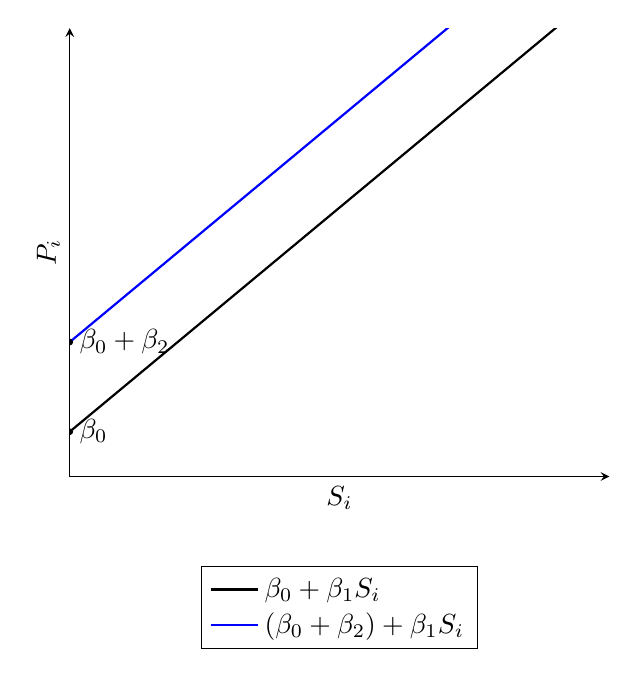
\begin{tikzpicture}
		\begin{axis}[axis lines = left, xmin = 0, ymin = 0, xmax = 10, ymax = 10, xlabel = $S_i$, ylabel = $P_i$, ticks=none, legend style={at={(0.5,-0.2)},anchor=north,legend cell align=left}]
			\addplot[domain=0:10,black, thick]{x+1};
			\addlegendentry{$\beta_0+\beta_1 S_i$}
			\addplot[domain=0:10,blue, thick]{x+3};
			\addlegendentry{$(\beta_0+\beta_2)+\beta_1 S_i$}
			\draw(axis cs:0,1)[fill]circle(1pt)node[right]{$\beta_0$};
			\draw(axis cs:0,3)[fill]circle(1pt)node[right]{$\beta_0+\beta_2$};
		\end{axis}
	\end{tikzpicture}
\end{center}

\section{Slope Dummy Variable}
\begin{align}
	P_i = \beta_0 + \beta_1 S_1 + \beta_2 (S_i \cdot D_i) + \epsilon_i\\
	E(P_i) =
	\begin{cases}
		\hat{\beta_0} + \left(\hat{\beta_1}+\hat{\beta_2} \right)S_i, &D_i = 1\\
		\hat{\beta_0} + \hat{\beta_1}S_i, &D_i = 0
	\end{cases}
\end{align}

\begin{center}
	\begin{tikzpicture}
		\begin{axis}[axis lines = left, xmin = 0, ymin = 0, xmax = 10, ymax = 10, xlabel = $S_i$, ylabel = $P_i$, ticks=none, legend style={at={(0.5,-0.2)},anchor=north,legend cell align=left}]
			\addplot[domain=0:10,black, thick]{0.5 * x+1};
			\addlegendentry{$\beta_0+\beta_1 S_i$}
			\addplot[domain=0:10,blue, thick]{x+1};
			\addlegendentry{$\beta_0+(\beta_1+\beta_2) S_i$}
			\draw(axis cs:0,1)[fill]circle(1pt)node[right]{$\beta_0$};
		\end{axis}
	\end{tikzpicture}
\end{center}


\section{Slope \& Dummy Variable}
\begin{align}
	P_i = \beta_0 + \beta_1 S_1 + \beta_2  D_i + \beta_3 S_i D_i + \epsilon_i\\
	E(P_i) =
	\begin{cases}
		(\hat{\beta_0} + \hat{\beta_2}) + \left(\hat{\beta_1}+\hat{\beta_3} \right)S_i, &D_i = 1\\
		\hat{\beta_0} + \hat{\beta_1}S_i, &D_i = 0
	\end{cases}
\end{align}

\begin{center}
	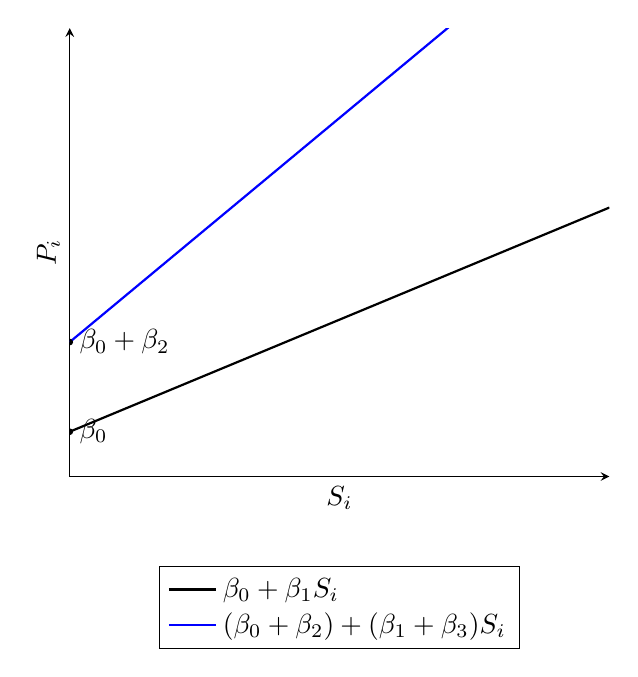
\begin{tikzpicture}
		\begin{axis}[axis lines = left, xmin = 0, ymin = 0, xmax = 10, ymax = 10, xlabel = $S_i$, ylabel = $P_i$, ticks=none, legend style={at={(0.5,-0.2)},anchor=north,legend cell align=left}]
			\addplot[domain=0:10,black, thick]{0.5 * x+1};
			\addlegendentry{$\beta_0+\beta_1 S_i$}
			\addplot[domain=0:10,blue, thick]{x+3};
			\addlegendentry{$(\beta_0+\beta_2)+(\beta_1+\beta_3) S_i$}
			\draw(axis cs:0,1)[fill]circle(1pt)node[right]{$\beta_0$};
			\draw(axis cs:0,3)[fill]circle(1pt)node[right]{$\beta_0+\beta_2$};
		\end{axis}
	\end{tikzpicture}
\end{center}

\section{Multi-Categories Dummy Variable}
\begin{align}
	P_0 = b_0 \begin{pmatrix} 1 \\ 1 \\ 1\end{pmatrix} + \underbrace{b_1 \begin{pmatrix} 1 \\ 0 \\ 0\end{pmatrix} + b_2 \begin{pmatrix} 0 \\ 1 \\ 0\end{pmatrix} +b_3 \begin{pmatrix} 0 \\ 0 \\ 1\end{pmatrix}}_{\text{Leads to Perfect Multicollinearlity}}
\end{align}
\subsubsection{Alternatives}
\begin{itemize}
	\item $B_n$ captures the mean of each category, but F-Test is impossible\begin{align} y = \beta_1 D_{1i} + \beta_2 D_{2i} + \beta_3 D_{3i}\end{align}
	\item Computer drops automatically drops a variable \begin{align} y = \beta_0 + \beta_1 D_{1i} + \beta_2 D_{2i} + \beta_3 D_{3i} \end{align}
	\item Manually dropping a variable \begin{align} y = \beta_0 + \beta_1 D_{1i} + \beta_2 D_{2i} \end{align}
\end{itemize}

\chapter{Logistic Regression}
For $Y_i \in \lbrace 0,1 \rbrace$:
\begin{align}
	z_k &= \beta_0 + \sum_{j=1}^{n} \beta_{jk} x_j + \epsilon_k, \beta_j \rightarrow \text{Logit Coefficient}\\
	p &= \dfrac{\exp^{k}}{1+\exp^{k}} = \dfrac{1}{1+\exp^{-k}}
\end{align}
where $p$ is the probability of $y=1$.

%End of Chapter------------------------------------------------

\part{Trigonometry}
\chapter{Circular Trigonometric Functions}
\begin{table}[htbp]
	\centering
	\begin{tabular}{c c c c}
		\toprule
		$\theta$&$\sin \theta$&$\cos \theta$&$\tan \theta$\\
		\midrule
		$\ang{0}$&$0$&$1$&$0$\\
		$\ang{15}$&$\frac{1}{4}$&$\frac{1}{4(2-\sqrt{3})}$&$2-\sqrt{3}$\\
		$\ang{18}$&$\frac{\sqrt{5}-1}{4}$&$\frac{\sqrt{10+2\sqrt{5}}}{4}$&$\frac{\sqrt{5}-1}{\sqrt{10+2\sqrt{5}}}$\\
		$\ang{30}$&$\frac{1}{2}$&$\frac{\sqrt{3}}{2}$&$\frac{1}{\sqrt{3}}$\\
		$\ang{36}$&$\frac{\sqrt{5}+1}{4}$&$\frac{\sqrt{10-2\sqrt{5}}}{4}$&$\frac{\sqrt{5}+1}{\sqrt{10-2\sqrt{5}}}$\\
		$\ang{45}$&$\frac{1}{\sqrt{2}}$&$\frac{1}{\sqrt{2}}$&$1$\\
		$\ang{60}$&$\frac{1}{\sqrt{3}}$&$\frac{1}{2}$&$\sqrt{3}$\\
		$\ang{72}$&$\frac{\sqrt{10+2\sqrt{5}}}{4}$&$\frac{\sqrt{5}-1}{4}$&$\frac{\sqrt{10+2\sqrt{5}}}{\sqrt{5}-1}$\\
		$\ang{90}$&$1$&$0$&$\infty$\\
		\hline
	\end{tabular}
	\caption{Trigonometric Ratios of Standard Angles}
	\label{table1}
\end{table}

For any given triangle:
\begin{equation}
	\dfrac{a}{\sin A}=\dfrac{b}{\sin B}=\dfrac{c}{\sin C}=2R
\end{equation}, where $2R$ is the radius of circumcircle.

\section{Negative Angle Formula}
\begin{align}
	\sin (-\theta)=-\sin \theta\\
	\cos (-\theta)=\cos \theta\\
	\tan (-\theta)=-\tan \theta\\
	\csc (-\theta)=-\csc \theta\\
	\sec (-\theta)=\sec \theta\\
	\cot (-\theta)=-\cot \theta
\end{align}


\section{Sum of Angles Formula}
\begin{align}
	\sin (A+B)=\sin A\cos B+\cos A\sin B\\
	\cos (A+B)=\cos A\cos B-\sin A\sin B\\
	\tan (A+B)=\dfrac{\tan A+\tan B}{1-\tan A\tan B}
\end{align}


\section{Difference of Angles Formula}
\begin{align}
	\sin (A-B)=\sin A\cos B-\cos A\sin B\\
	\cos (A-B)=\cos A\cos B+\sin A\sin B\\
	\tan (A-B)=\dfrac{\tan A-\tan B}{1+\tan A\tan B}
\end{align}


\section{Multiples and Sub-multiples of $\pi$ and $\frac{\pi}{2}$}
\begin{align}
	\forall k \in \mathbb{Z}\nonumber\\
	\sin \left((4k+1)\dfrac{\pi}{2}\right)=1\\
	\sin \left((4k-1)\dfrac{\pi}{2}\right)=-1\\
	\sin k\pi=0\\
	\sin \left((2k+1)\dfrac{\pi}{2}\right)=0\\
	\sin \left((2k-1)\dfrac{\pi}{2}\right)=0\\
	\sin k\pi=(-1)^k
\end{align}


\section{$\left(\frac{\pi}{2}\pm\theta\right)$ Formula}
\begin{align}
	\sin \left(\dfrac{\pi}{2}-\theta\right)=\cos \theta\\
	\sin \left(\dfrac{\pi}{2}+\theta\right)=\cos \theta\\
	\hline
	\cos \left(\dfrac{\pi}{2}-\theta\right)=\sin \theta\\
	\cos \left(\dfrac{\pi}{2}+\theta\right)=-\sin \theta\\
	\hline
	\tan \left(\dfrac{\pi}{2}-\theta\right)=\cot \theta\\
	\tan \left(\dfrac{\pi}{2}+\theta\right)=-\cot \theta\\
	\hline
	\cot \left(\dfrac{\pi}{2}-\theta\right)=\tan \theta\\
	\cot \left(\dfrac{\pi}{2}+\theta\right)=-\tan \theta\\
	\hline
	\csc \left(\dfrac{\pi}{2}-\theta\right)=\sec \theta\\
	\csc \left(\dfrac{\pi}{2}+\theta\right)=\sec \theta\\
	\hline
	\sec \left(\dfrac{\pi}{2}-\theta\right)=\csc \theta\\
	\sec \left(\dfrac{\pi}{2}+\theta\right)=-\csc \theta
\end{align}


\section{$\left(\frac{\pi}{4}\pm\theta\right)$ Formula}
\begin{align}
	\tan \left(\frac{\pi}{4}+\theta\right)=\dfrac{1+\tan \theta}{1-\tan \theta}\\
	\tan \left(\frac{\pi}{4}-\theta\right)=\dfrac{1-\tan \theta}{1+\tan \theta}
\end{align}


\section{Trigonometric Identities}
\begin{align}
	\sin^2 \theta+\cos^2 \theta=1\\
	\tan^2 \theta+1=\sec^2 \theta\\
	\cot^2 \theta+1=\csc^2 \theta
\end{align}


\section{Double Angle Formula}
\begin{equation}
	\begin{aligned}
		\begin{split}
			\sin 2\theta &=& 2\sin \theta \cos \theta\\
			&=&\dfrac{2 \tan \theta}{1+\tan^2 \theta}
		\end{split}
	\end{aligned}
\end{equation}
\begin{equation}
	\begin{aligned}
		\begin{split}
			\cos 2\theta &=& \cos^2 \theta -\sin^2 \theta\\
			&=&2\cos^2 \theta-1\\
			&=&1-2\sin^2 \theta\\
			&=&\dfrac{1-\tan^2 \theta}{1+\tan^2 \theta}
		\end{split}
	\end{aligned}
\end{equation}
\begin{equation}
	\tan 2\theta=\dfrac{2 \tan \theta}{1-\tan^2 \theta}
\end{equation}


\section{Triple Angle Formula}
\begin{align}
	\sin 3\theta=3\sin \theta-4 \sin^3 \theta\\
	\cos 3\theta=4\cos^3 \theta-3 \cos \theta\\
	\tan 3\theta=\dfrac{3\tan \theta -\tan^3 \theta}{1-3\tan^3 \theta}
\end{align}


\section{Sum and Product of Two Ratios}
For $A>B$:
\begin{align}
	\sin A+\sin B=2 \sin \left(\frac{A+B}{2}\right)\cos \left(\frac{A-B}{2}\right)\\
	\sin A-\sin B=2 \cos \left(\frac{A+B}{2}\right)\sin \left(\frac{A-B}{2}\right)\\
	2\sin A\cos B=\sin(A+B)+\sin(A-B)\\
	2\cos A\sin B=\sin(A+B)-\sin(A-B)\\
	\cos A+\cos B=2 \cos \left(\frac{A+B}{2}\right)\cos \left(\frac{A-B}{2}\right)\\
	\cos A-\cos B=-2 \sin \left(\frac{A+B}{2}\right)\sin \left(\frac{A-B}{2}\right)\\
	2 \cos A\cos B=\cos (A+B)+\cos (A-B)\\
	2 \cos A\sin B=\cos (A+B)-\cos (A-B)\\
	\sin (A-B)\sin(A+B)=\sin^2 A-\sin^2 B\\
	\cos (A-B)\cos(A+B)=\cos^2 A-\sin^2 B\\
	\tan (A-B)\tan(A+B)=\dfrac{\tan^2 A-\tan^2 B}{1-\tan^2 A\tan^2 B}
\end{align}


\section{General Solutions}
If $\sin \theta=\sin \alpha$:
\begin{equation}
	\theta=n\pi+(-1)^n\alpha
\end{equation}
$n\in\mathbb{Z}$

If $\cos \theta=\cos \alpha$:
\begin{equation}
	\theta=2n\pi\pm\alpha
\end{equation}
$n\in\mathbb{Z}$

If $\tan \theta=\tan \alpha$:
\begin{equation}
	\theta=n\pi\pm\alpha
\end{equation}
$n\in\mathbb{Z}$


\section{Taylor Series Expansion of Trigonometric Ratios}
\begin{align}
	\sin x=x-\dfrac{x^3}{3!}+\dfrac{x^5}{5!}-\cdots\infty=\sum_{i=1}^\infty (-1)^{i+1}\dfrac{x^{2i-1}}{(2i-1)!}\\
	\cos x=1-\dfrac{x^2}{2!}+\dfrac{x^4}{4!}-\cdots\infty=\sum_{i=0}^\infty (-1)^i\dfrac{x^{2i}}{(2i)!}
\end{align}

\large{\chapter{Inverse Circular Trigonometric Function}}
\section{Definition of Inverse Circular Trigonometric Function}
\subsection{For $\sin x$}
$y=\arcsin x$ iff $x=\sin y$, then:
\begin{enumerate}
	\item $y \in [-\frac{\pi}{2},\frac{\pi}{2}]$
	\item domain of $x \in [-1,1]$
	\item $\sin(\arcsin x)=x,\forall x\in[-1,1]$
	\item $\arcsin(\sin y)=y, \forall y\in [-\frac{\pi}{2},\frac{\pi}{2}]$
	\item $\sin x$ is a strictly increasing in the domain $[-\frac{\pi}{2},\frac{\pi}{2}]$ and one-one.
\end{enumerate}

\subsection{For $\cos x$}
$y=\arccos x$ iff $x=\cos y$, then:
\begin{enumerate}
	\item $y \in [0,\pi]$
	\item domain of $x \in [-1,1]$
	\item $\cos(\arccos x)=x,\forall x\in[-1,1]$
	\item $\arccos(\cos y)=y, \forall y\in [0,\pi]$
	\item $\cos x$ is a strictly decreasing in the domain $[0,\pi]$ and one-one.
\end{enumerate}

\subsection{For $\tan x$}
$y=\arctan x$ iff $x=\tan y$, then:
\begin{enumerate}
	\item $y \in [-\frac{\pi}{2},\frac{\pi}{2}]$
	\item domain of $x \in \mathbb{R}$
	\item $\tan(\arctan x)=x,\forall x\in\mathbb{R}$
	\item $\arctan(\tan y)=y, \forall y\in [-\frac{\pi}{2},\frac{\pi}{2}]$
	\item $\tan x$ is a strictly increasing in the domain $[-\frac{\pi}{2},\frac{\pi}{2}]$ and one-one.
\end{enumerate}

\subsection{For $\cot x$}
$y=\cot^{-1} x$ iff $x=\cot y$, then:
\begin{enumerate}
	\item $y \in (0,\pi)$
	\item domain of $x \in \mathbb{R}$
	\item $\cot(\cot^{-1} x)=x,\forall x\in\mathbb{R}$
	\item $\cot^{-1}(\cot y)=y, \forall y\in (0,\pi)$
	\item $\cot x$ is a strictly decreasing in the domain $(0,\pi)$ and one-one.
\end{enumerate}

\subsubsection{For $\sec x$}
$y=\sec^{-1} x$ iff $x=\sec y$
\begin{enumerate}
	\item $y\in\left\lbrace [0,\frac{\pi}{2})\cup(\frac{\pi}{2},\pi]\right\rbrace$
	\item $x\in\left\lbrace(-\infty,-1]\cup[1,\infty)\right\rbrace$
	\item $\sec(\sec^{-1}x)=x,\forall \lvert x \rvert \geq 1$
	\item $\sec^{-1}(\sec y)=y, \forall y \in \left\lbrace [0,\frac{\pi}{2})\cup(\frac{\pi}{2},\pi]\right\rbrace$
\end{enumerate}

\subsection{For $\csc x$}
$y=\csc^{-1} x$ iff $x=\csc y$
\begin{enumerate}
	\item $y\in\left\lbrace [-\frac{\pi}{2},0)\cup(0,\frac{\pi}{2}]\right\rbrace$
	\item $x\in\left\lbrace(-\infty,-1]\cup[1,\infty)\right\rbrace$
	\item $\csc(\csc^{-1}x)=x,\forall \lvert x \rvert \geq 1$
	\item $\csc^{-1}(\csc y)=y, \forall y \in \left\lbrace [-\frac{\pi}{2},0)\cup(0,\frac{\pi}{2}]\right\rbrace$
\end{enumerate}

\section{Negative Arguments}
\begin{align}
	\arcsin (-x)=-\arcsin x\\
	\arctan (-x)=-\arctan x\\
	\csc^{-1} (-x)=-\csc^{-1} x\\
	\arccos (-x)=\pi-\arccos x\\
	\cot^{-1} (-x)=\pi-\cot^{-1} x\\
	\sec^{-1} (-x)=\pi-\sec^{-1} x
\end{align}

\section{Reciprocal Relations}
\begin{align}
	\csc^{-1} x=\arcsin \dfrac{1}{x}\\
	\sec^{-1} x=\arccos \dfrac{1}{x}\\
	\sec^{-1} x=\begin{cases}
		\arctan \dfrac{1}{x}, x>0\\
		\pi+\arctan \dfrac{1}{x}, x<0
	\end{cases}
\end{align}

\section{I.T.F. Identities}
\begin{align}
	\arcsin x+\arccos x=\dfrac{\pi}{2}, \lvert x \rvert \leq 1\\
	\arctan x+\cot^{-1} x=\dfrac{\pi}{2}, x\in\mathbb{R}\\
	\sec^{-1} x+\csc^{-1} x=\dfrac{\pi}{2}, \lvert x \rvert \geq 1
\end{align}

\section{Sum of Two Angles}
\begin{align}
	\arctan x+\arctan y=\arctan \left(\dfrac{x+y}{1-xy}\right)\\
	\arcsin x+\arcsin y=\arcsin (y\sqrt{1-x^2}+x\sqrt{1-y^2})\\
	\arccos x+\arccos y=\arccos (xy-\sqrt{1-x^2}\sqrt{1-y^2})
\end{align}

\section{Difference of Two Angles}
\begin{align}
	\arctan x-\arctan y=\arctan \left(\dfrac{x-y}{1+xy}\right)\\
	\arcsin x-\arcsin y=\arcsin (x\sqrt{1-y^2}-y\sqrt{1-x^2})\\
	\arccos x-\arccos y=\arccos (xy+\sqrt{1-x^2}\sqrt{1-y^2})
\end{align}

\section{Interconversion of Ratios}
\begin{equation}
	\begin{aligned}
		\begin{split}
			\arcsin x & = & \arccos \sqrt{1-x^2}\\
			& = & \arctan \left(\dfrac{x}{\sqrt{1-x^2}}\right)
		\end{split}
	\end{aligned}
\end{equation}

\begin{equation}
	\begin{aligned}
		\begin{split}
			\arccos x & = & \arcsin \sqrt{1-x^2}\\
			& = & \arctan \left(\dfrac{\sqrt{1-x^2}}{x}\right)
		\end{split}
	\end{aligned}
\end{equation}

\begin{equation}
	\begin{aligned}
		\begin{split}
			2\arctan x & = & \arcsin\left(\dfrac{2x}{1+x^2}\right)\\
			& = & \arccos \left(\dfrac{1-x^2}{1+x^2}\right)\\
			& = & \arctan \left(\dfrac{2x}{1-x^2}\right)
		\end{split}
	\end{aligned}
\end{equation}

\section{Miscellaneous Relations}
\begin{align}
	\cos(\arcsin x)=\sin(\arccos x)=\sqrt{1-x^2}\\
	\arctan x=\frac{\pi}{2}-\arctan\left(\frac{1}{x}\right), x>1
\end{align}
%End of Chapter------------------------------------------------
\large{\chapter{Hyperbolic Trigonometric Function}}
\section{Definition}
Hyperbolic trigonometric functions are defined such that $(\cosh t,\sinh t)$ form the right half of an equilateral hyperbola. The functions are defined as follows:
\begin{align}
	\sinh x=\dfrac{\exp(x)-\exp(-x)}{2}\\
	\cosh x=\dfrac{\exp(x)+\exp(-x)}{2}\\
	\tanh x=\dfrac{\sinh x}{\cosh x}=\dfrac{\exp(x)-\exp(-x)}{\exp(x)+\exp(-x)}\\
	\coth x=\dfrac{1}{\tanh x}=\dfrac{\exp(x)+\exp(-x)}{\exp(x)-\exp(-x)}\\
	csch x=\dfrac{1}{\sinh x}=\dfrac{2}{\exp(x)-\exp(-x)}\\
	sech x=\dfrac{1}{\cosh x}=\dfrac{2}{\exp(x)+\exp(-x)}
\end{align}

\section{Identities}
\begin{align}
	\coth^2 x-\sinh^2 x=1\\
	\tanh^2 x+sech^2 x=1\\
	\coth^2 x-csch^2 x=1
\end{align}

\section{Inverse Hyperbolic Function}
\begin{align}
	\sinh^{-1} z= \ln(z+\sqrt{z^2+1})\\
	\cosh^{-1} z= \ln(z\pm\sqrt{z^2-1})\\
	\tanh^{-1} z= \dfrac{1}{2}\ln\left(\dfrac{1+z}{1-z}\right)\\
	\coth^{-1} z= \dfrac{1}{2}\ln\left(\dfrac{z+1}{z-1}\right)\\
	csch^{-1} z= \ln\left(\dfrac{1\pm\sqrt{z^2+1}}{z}\right)\\
	sech^{-1} z= \ln\left(\dfrac{1\pm\sqrt{1-z^2}}{2}\right)
\end{align}

\section{Relation to Circular Trigonometric Functions}
\begin{align}
	\sinh (z)=-i\sin (iz)\\
	\coth (z)= \cos (iz)\\
	\tanh (z)=-i \tan (iz)\\
	csch (z)=i\csc (iz)\\
	sech (z)=\sec (iz)\\
	\coth (z)=i\cot (iz)
\end{align}
%End of Chapter----------------------------------------------------

\part{Calculus}
\large{\chapter{Limits}}
\begin{align}
	\lim_{x\to0} \dfrac{\sin x}{x}=1\\
	\lim_{x\to0} \dfrac{\tan x}{x}=1\\
	\lim_{x\to0} \cos x=1\\
	\lim_{x\to a} \dfrac{x^n-a^n}{x-a}=na^{n-1}\\
	\lim_{x\to a} f(x)g(x)=\lim_{x\to a} f(x)\lim_{x\to a} g(x)\\
	\lim_{x\to a} \dfrac{f(x)}{g(x)}=\dfrac{\lim_{x\to a} f(x)}{\lim_{x\to a} g(x)}, \lim_{x\to a} g(x) \neq 0\\
	\lim_{x\to0} \exp(x)=1\\
	\lim_{x\to a} \exp(x)=\exp(c)\\
	\lim_{x\to0} \dfrac{\exp(x)-1}{x}=1\\
	\lim_{x\to a} c^x=c^a
\end{align}
\begin{align}
	\lim_{x\to a} \ln x=\ln a\\
	\lim_{x\to0} (1+x)^{\frac{1}{x}}=e\\
	\lim_{x\to0} \dfrac{\ln (1+x)}{x}=1\\
	\lim_{x\to0} \dfrac{a^x-1}{x}=\ln a\\
	\lim_{n\to\infty} \dfrac{x^n}{n!}=0, \forall x\in\mathbb{R}
\end{align}

\section{L'Hospital Rule}
If:
\begin{equation}
	L=\lim_{x\to a} \dfrac{f(x)}{g(x)}\nonumber
\end{equation}
is such that $f(a)=0$ and $g(a)=0$, or $f(a)=\infty$ and $g(a)=\infty$, then:
\begin{equation}
	L=\lim_{x\to a} \dfrac{f'(x)}{g'(x)}\nonumber
\end{equation}
%End of Chapter-----------------------------------------------------------------------------------
\chapter{Differentiation}
\section{Differentiation by First Principle}
\begin{equation}
	\dfrac{df(x)}{dx}=\lim_{h\to0} \dfrac{f(x+h)-f(x)}{h}
\end{equation}

\section{Standard Differentiation Formulae}
\begin{align}
	\dfrac{dk}{dx}=0\\
	\dfrac{dx^n}{dx}=nx^{n-1}\\
	\dfrac{da^x}{dx}=\ln a\cdot a^x
\end{align}
\begin{align}
	\dfrac{d\exp(x)}{dx}=\exp(x)\\
	\dfrac{d\ln x}{dx}=\dfrac{1}{x}\\
	\dfrac{d\sqrt{x}}{dx}=\dfrac{1}{2\sqrt{2}}\\
\end{align}
\subsection{Circular Trigonometric Functions}
\begin{align}
	\dfrac{d\sin x}{dx}& = \cos x\\
	\dfrac{d\cos x}{dx}& = -\sin x\\
	\dfrac{d\tan x}{dx}& = \sec^2 x\\
	\dfrac{d\sec x}{dx}& = \sec x\tan x\\
	\dfrac{d\csc x}{dx}& = -\csc x\cot x\\
	\dfrac{d\cot x}{dx}& = -\csc^2 x
\end{align}
\subsection{Inverse Circular Trigonometric Functions}
\begin{align}
	\dfrac{d\arcsin x}{dx}=\dfrac{1}{\sqrt{1-x^2}}, \lvert x \rvert \leq 1\\
	\dfrac{d\arccos x}{dx}=-\dfrac{1}{\sqrt{1-x^2}}, \lvert x \rvert \leq 1\\
	\dfrac{d\arctan x}{dx}=\dfrac{1}{1+x^2}\\
	\dfrac{d\cot^{-1} x}{dx}=-\dfrac{1}{1+x^2}\\
	\dfrac{d\sec^{-1} x}{dx}=\dfrac{1}{x\sqrt{x^2-1}}, \lvert x \rvert \geq 1\\
	\dfrac{d\csc^{-1} x}{dx}=-\dfrac{1}{x\sqrt{x^2-1}}, \lvert x \rvert \geq 1
\end{align}

\subsection{Hyperbolic Trigonometric Function}
\begin{align}
	\dfrac{d\sinh x}{dx}=\cosh x\\
	\dfrac{d\cosh x}{dx}=\sinh x\\
	\dfrac{d\tanh x}{dx}=1-\tanh^2 x=sech^2 (x)\\
	\dfrac{d\coth x}{dx}=1-\coth^2 x=-csch^2 (x)\\
	\dfrac{d[sech(x)]}{dx}=-\tanh x \text{ sech}x\\
	\dfrac{d[csch(x)]}{dx}=-\coth x \text{ csch}x
\end{align}

\subsection{Inverse Hyperbolic Trigonometric Function}
\begin{align}
	\dfrac{d\sinh x}{dx}=\dfrac{1}{\sqrt{x^2+1}}\\
	\dfrac{d\cosh x}{dx}=\dfrac{1}{\sqrt{x^2-1}}\\
	\dfrac{d\tanh x}{dx}=\dfrac{1}{1-x^2}\\
	\dfrac{d\coth x}{dx}=\dfrac{1}{1-x^2}\\
	\dfrac{d[sech(x)]}{dx}=\dfrac{1}{x\sqrt{1-x^2}}\\
	\dfrac{d[csch(x)]}{dx}=\dfrac{1}{\lvert x \rvert \sqrt{1+x^2}}
\end{align}

\section{Rules of Differentiation}
\begin{align}
	\dfrac{d[cf(x)]}{dx}=c\dfrac{df(x)}{dx}\\
	\dfrac{d[f_1(x)+f_2(x)]}{dx}=\dfrac{d[f_1(x)]}{dx}+\dfrac{d[f_2(x)]}{dx}\\
	\dfrac{d[f_1f_2]}{dx}=f_1f_2'+f_2f_1'\\
	\dfrac{d\left(\frac{f_1}{f_2}\right)}{dx}=\dfrac{f_2f_1'-f_1f_2'}{f_2^2}
\end{align}

\section{Chain Rule}
If two functions are defined as $z=f(y)$ and $y=g(x)$:
\begin{equation}
	\dfrac{dz}{dx}=\dfrac{dz}{dy}\cdot\dfrac{dy}{dx}
\end{equation}
If two functions are defined as $x=f(\theta)$ and $y=g(\theta)$:
\begin{equation}
	\dfrac{d^2y}{dx^2}=\left[\dfrac{d}{d\theta}\left(\dfrac{\frac{dy}{d\theta}}{\frac{dx}{d\theta}}\right)\right]\dfrac{d\theta}{dx}
\end{equation}
%End of Chapter--------------------------------------------------------------
\chapter{Successive Differentiation}
\begin{align}
	D^n (ax+b)^m=m(m-1)\cdots(m-n+1) a^n (ax+b)^{m-n}\\
	D^n \left(\dfrac{1}{ax+b}\right)=\dfrac{(-1)^n n!a^n}{(ax+b)^{n+1}}\\
	D^n \ln(ax+b)=\dfrac{(-1)^{n-1} (n-1)!a^n}{(ax+b)^n}, n \geq 2\\
	D^n (a^{mx})=m^n (\ln a)^n a^{mx}\\
	D^n (e^{mx})=m^n e^{mx}\\
	D^n \sin (ax+b)=a^n \sin(ax+b+n\frac{\pi}{2})\\
	D^n \cos (ax+b)=a^n \cos(ax+b+n\frac{\pi}{2})\\
	D^n [e^{ax} \sin(bx+c)]=(a^2+b^2)^{\frac{n}{2}} e^{ax} \sin(bx+c+n\arctan\frac{b}{a})\\
	D^n [e^{ax} \cos(bx+c)]=(a^2+b^2)^{\frac{n}{2}} e^{ax} \cos(bx+c+n\arctan\frac{b}{a})
\end{align}


\section{Leibnitz's Theorem}
For two functions $u$ and $v$ of $x$, the successive differentiation of their product is defined as:
\begin{equation}
	\begin{aligned}
		\begin{split}
			(uv)_n & = &^nC_0 u_n v+^nC_1 u_{n-1} v_1+\cdots+^nC_0 u v_n\\
			& = & \sum_{i=0}^n {^nC_i} u_{n-i} v_i
		\end{split}
	\end{aligned}
\end{equation}

\large{\chapter{Partial Derivative}}
If $f(x,y)$ is a function of $(x,y)$, then $\dfrac{\delta f(x,y)}{\delta x}$ is the differentiation of $f(x,y)$ w.r.t. $x$, keeping all other parameters constant.
\section{Chain Rule}
If $f$ is a function of $u$ and $v$, which are functions of $x$ and $y$, then:
\begin{equation}
	\dfrac{\delta f}{\delta x}=\dfrac{\delta f}{\delta u}\dfrac{\delta u}{\delta x}+\dfrac{\delta f}{\delta v}\dfrac{\delta v}{\delta x}
\end{equation}
\begin{equation}
	\dfrac{\delta f}{\delta y}=\dfrac{\delta f}{\delta u}\dfrac{\delta u}{\delta y}+\dfrac{\delta f}{\delta v}\dfrac{\delta v}{\delta y}
\end{equation}
If $f$ is a function of $x$ and $y$, which are functions of $t$, then:
\begin{equation}
	\dfrac{df}{dt}=\dfrac{\delta f}{\delta x}\dfrac{dx}{dt}+\dfrac{\delta f}{\delta y}\dfrac{dy}{dt}
\end{equation}

\section{Euler's Theorem}
For a homogeneous function \footnote{Homogeneous functions are defined as $f(ax,ay)=a^\kappa f(x,y)$, where $\kappa$ is the degree of homogeneity.\newline E.g. $f(x,y)=x^2+y^2$, then $f(tx,ty)=t^2(x^2+y^2$), and the degree of homogeneity is $2$.}, $f(x_i)$ of degree $n$:
\begin{equation}
	\sum x_i\dfrac{\delta f}{\delta x_i}=nf(x_i)
\end{equation}
%End of Chapter-------------------------------------------------------------
\chapter{Application of Differentiation}
\section{Rolle's Theorem}
For a function $f(x)$:
\begin{enumerate}
	\item is continuous in $[a,b]$
	\item is differentiable in $(a,b)$
	\item $f(a)=f(b)$,
\end{enumerate}
then there exists a point $x=c$ such that $f'(c)=0$, $c\in(a,b)$


\section{Mean Value Theorem or LaGrange's Theorem}
For a function $f(x)$:
\begin{enumerate}
	\item is continuous in $[a,b]$
	\item is differentiable in $(a,b)$,
\end{enumerate}
then there exists a point $x=c$ such that $f'(c)=\dfrac{f(b)-f(a)}{b-a}$, $c\in(a,b)$, i.e., the tangent is parallel to the line joining the the points $(a,f(a))$ and $(b,f(b))$.


\section{Cauchy's Mean Value Theorem}
For a function $f(x)$ and $g(x)$:
\begin{enumerate}
	\item are continuous in $[a,b]$
	\item are differentiable in $(a,b)$
	\item $g'(x)\neq 0$ in $(a,b)$,
\end{enumerate}
then there exists a point $c\in(a,b)$, such that $\dfrac{f(x)}{g(x)}=\dfrac{f(b)-f(a)}{g(b)-g(a)}$.

\section{Maxima and Minima}
\subsection{Maxima}
For the local maxima of a function $f(x)$:
\begin{enumerate}
	\item $f'(c)=0$ and
	\begin{align}
		\lim_{\epsilon\to c^{-}} f'(\epsilon)>0\nonumber\\
		\lim_{\epsilon\to c^{+}} f'(\epsilon)<0\nonumber
	\end{align}
	\begin{center}
		OR
	\end{center}
	\item $f'(c)=0$ and $f''(x)<0$,
\end{enumerate}
then $f(c)$ is the local maxima point of the function $f(x)$.

\subsection{Minima}
For the local minima of a function $f(x)$:
\begin{enumerate}
	\item $f'(c)=0$ and
	\begin{align}
		\lim_{\epsilon\to c^{-}} f'(\epsilon)<0\nonumber\\
		\lim_{\epsilon\to c^{+}} f'(\epsilon)>0\nonumber
	\end{align}
	\begin{center}
		OR
	\end{center}
	\item $f'(c)=0$ and $f''(x)>0$,
\end{enumerate}
then $f(c)$ is the local minima point of the function $f(x)$.


\section{Taylor's Theorem}
For a function which is differentiable $n$ times:
\begin{equation}
	f(a+h)=f(a)+hf'(a)+\dfrac{h^2}{2!}f''(a)+\cdots+\dfrac{h^{n-1}}{(n-1)!} f^{n-1}(a)+\dfrac{h^n}{x!}R_n
\end{equation}
where $R_n$ is the remainder term.

\subsection{Remainder Term}
\subsubsection{LeGrange's Form}
\begin{equation}
	R_n=f^n (a+\theta h), \theta \in (0,1)
\end{equation}

\subsubsection{Cauchy's Form}
\begin{equation}
	R_n=n(1-\theta)^{n-1}f^n(a+\theta h), \theta \in (0,1)
\end{equation}

\subsection{Conditions for Validity of Expansion}
For validity of Taylor Expansion,the condition
\begin{equation}
	\lim_{n\to\infty} R_n=0
\end{equation}
needs to be satisfied either where $R_n$ is the remainder term in either LeGrange's Form or Cauchy's Form. If the condition is satisfied in a certain domain, then the expansion is valid within that domain only.

\subsection{Taylor's Theorem for Two Variables}
\begin{equation}
	\begin{aligned}
			f(a+x,b+y)& = &f(x,y)+\left( a\dfrac{\delta}{\delta x}+b\dfrac{\delta}{\delta y}\right)f (x,y)+&\\
			& &\dfrac{1}{2!}\left( a^2\dfrac{\delta^2}{\delta x^2}+b^2\dfrac{\delta^2}{\delta y^2}\right) f(x,y)+\cdots+&\\
			& &\dfrac{1}{n!}\left( a^n\dfrac{\delta^n}{\delta x^n}+b^n\dfrac{\delta^n}{\delta y^n}\right) f(x+\theta a,y+\theta b), \theta \in (0,1)
	\end{aligned}
\end{equation}


\section{Maclaurin's Series}
\begin{equation}
	\begin{aligned}
			f(x)&=&f(0)+xf'(0)+\dfrac{1}{2!}x^2f''(0)+\dfrac{1}{3!}x^3f'''(0)+\cdots\infty&\\
			&=& \sum_{i=0}^\infty \dfrac{1}{i!} x^i f^i(0)
	\end{aligned}
\end{equation}

\subsection{Maclaurin's Series with Two Variables}
\begin{equation}
	\begin{aligned}
			f(a,b)&=&f(0,0)+\left(a\dfrac{\delta}{\delta x}+b\dfrac{\delta}{\delta x}\right)f(0,0)+&\\& &\dfrac{1}{2!}\left(a^2\dfrac{\delta^2}{\delta x^2}+b^2\dfrac{\delta^2}{\delta x^2}\right)f(0,0)+\cdots\infty&\\
			& = & \sum_{i=0}^\infty \dfrac{1}{n!}\left(a^i\dfrac{\delta^i}{\delta x^i}+b^i\dfrac{\delta^i}{\delta x^i}\right)f(0,0)
	\end{aligned}
\end{equation}


\section{Curvature}
Curvature is the rate of change of direction w.r.t. arc. Mathematically:
\begin{equation}
	\text{Curvature}=\dfrac{d(\text{direction})}{d(\text{arc})}\nonumber
\end{equation}
\begin{equation}
	\lim_{\Delta s \to 0} \dfrac{\Delta \psi}{\Delta s}=\dfrac{d\psi}{ds}
\end{equation}

\subsection{Radius of Curvature}
\subsubsection{Cartesian Form}
For a curve $y=f(x)$:
\begin{equation}
	\rho=\dfrac{(1+y'^2)^{\frac{3}{2}}}{y''}
\end{equation}
However, this formula fails for $y'\to\infty$.
\subsubsection{Parametric Form}
For a curve defined as $x=\phi(t)$ and $y=\psi(t)$:
\begin{equation}
	\rho=\dfrac{(\ddot{x}^2+\ddot{y}^2)^{\frac{3}{2}}}{x\ddot{y}-y\ddot{x}}
\end{equation}

\subsection{Newton's Formula}
\begin{enumerate}
	\item If the curve passes through origin, and the tangent at origin is the x-axis:
	\begin{equation}
		\rho=\lim_{^{x\to0}_{y\to0}} \dfrac{x^2}{2y}
	\end{equation}
	\item If the curve passes through origin, and the tangent at origin is the y-axis:
	\begin{equation}
		\rho=\lim_{^{x\to0}_{y\to0}} \dfrac{y^2}{2x}
	\end{equation}
	\item If the curve passes through origin and $ax+by+c=0$ is the tangent at origin:
	\begin{equation}
		\rho(0,0)=\dfrac{1}{2}\sqrt{a^2+b^2} \lim_{^{x\to0}_{y\to0}} \dfrac{a^2+y^2}{ax+by}
	\end{equation}
\end{enumerate}

\subsection{Tangent at Origin}
For a curve
\begin{equation}
	\sum c_i x^j y^k=0, i\in\mathbb{N}\text{ and }j,k\in\mathbb{Z}-\lbrace 0 \rbrace
\end{equation}
The curve passes through origin $\because c=0$. Then the lowest degree term equated to $x$ gives the tangent at origin.


\section{Asymptotes}
If the distance between a line $P$ and a curve $f(x)$, $s$ is such that $s\to0$, as $x\to\infty$, then $P$ is the asymptote of $f(x)$. For asymptotes not parallel to x-axis:\newline
Let $y=mx+c$ be the asymptote of the function $y=f(x)$, then:
\begin{align}
	m=\lim_{x\to\infty} \dfrac{y}{x}\\
	c=\lim_{x\to\infty} (y-mx)
\end{align}

\subsection{Asymptote of Algebraic Curves}
For an algebraic curve, passing through origin, defined as:
\begin{equation}
	\begin{aligned}
			(a_0x^n+a_1x^{n-1}y^1+a_2x^{n-2}y^2+\cdots+a_{n-1}xy^{n-1}+a_n y^n)+&\\
			(b_0x^{n-1}+b_1x^{n-2}y^1+b_2x^{n-3}y^2+\cdots+b_{n-1}xy^{n-2}+a_n y^{n-1})+&\\
			\cdots=0\nonumber
	\end{aligned}
\end{equation}
\begin{equation}
	\Rightarrow x^n\phi_n\left(\dfrac{y}{x}\right)+x^{n-1}\phi_{n-1}\left(\dfrac{y}{x}\right)+\cdots+x\phi_1\left(\dfrac{y}{x}\right)=0\nonumber
\end{equation}
The asymptote(s) defined as $y=mx+c$,
\begin{enumerate}
	\item $m$ is the solution for the equation
	\begin{equation}
		\phi_n(m)=0
	\end{equation}
	\item \begin{equation}
		c=-\dfrac{\phi_{n-1}(m)}{\phi_n (m)}
	\end{equation}
	where $c$ is a finite value.
\end{enumerate}

\large{\chapter{Integration}}
\section{General Formulae}
\footnote{A is the constant of integration in all cases}
\begin{align}
	\int nx^{n-1} dx=x^n+A\\
	\int x^n dx=\dfrac{1}{n+1}x^{n+1}+A\\
	\int e^x dx=e^x+A\\
	\int \dfrac{1}{x} dx=\ln x+A\\
	\int \ln x dx=x(\ln x-1)+A
\end{align}

\section{Circular Trigonometric Functions}
\begin{align}
	\int \sin x dx& = -\cos x+A\\
	\int \cos x dx& = \sin x+A\\
	\int \sec^2 x dx& = \tan x+A\\
	\int \csc^2 x dx& = -\cot x+A\\
	\int \sec x \tan x dx& = \sec x+A\\
	\int \csc x \cot x dx& = -\csc x+A\\
	\int \sec x dx& = \ln (\sec x+\tan x)+A\\
	\int \csc x dx& = -\ln (\csc x+\cot x)+A\\
	\int \tan x dx& = -\ln (\cos x)+A \nonumber \\
	& = \ln(\sec x)+A\\
	\int \cot x dx& = \ln (\sin x)+A
\end{align}

\section{Inverse Circular Trigonometric Function}
\begin{align}
	\int \dfrac{1}{\sqrt{1-x^2}}dx=\sin^{-1} x+A\\
	\int \dfrac{-1}{\sqrt{1-x^2}}dx=\cos^{-1} x+A\\
	\int \dfrac{1}{1+x^2}dx=\tan^{-1} x+A\\
	\int \dfrac{-1}{1+x^2}dx=\cot^{-1} x+A=-\tan^{-1} x+A\\
	\int \dfrac{1}{x\sqrt{x^2-1}}dx=\sec^{-1} x+A=-\csc^{-1} x+A\\
	\int \dfrac{-1}{x\sqrt{x^2-1}}dx=\csc^{-1} x+A=-\sec^{-1} x+A
\end{align}

\section{Standard Integrals}
\begin{align}
	\int \dfrac{dx}{\sqrt{a^2-x^2}}& = \sin^{-1} \dfrac{x}{a}+A\\
	\int \dfrac{dx}{\sqrt{x^2+a^2}}& = \ln (x+\sqrt{x^2+a^2})+A\\
	\int \dfrac{dx}{a^2+x^2}& = \dfrac{1}{a}\tan^{-1} \dfrac{x}{a}+A\\
	\int \dfrac{dx}{\sqrt{x^2-a^2}}& = \ln (x+\sqrt{x^2-a^2})+A\\
	\int \dfrac{dx}{x\sqrt{x^2-a^2}}& = \dfrac{1}{a} \sec^{-1} \dfrac{x}{a}+A\\
	\int \sqrt{a^2-x^2}dx& = \dfrac{x\sqrt{a^2-x^2}}{2}+\dfrac{a^2}{2}\sin^{-1} \dfrac{x}{a}+A\\
	\int \sqrt{a^2+x^2}dx& = \dfrac{x\sqrt{a^2+x^2}}{2}+\dfrac{a^2}{2}\ln (x+\sqrt{x^2+a^2})+A\\
	\int \sqrt{x^2-a^2}dx& = \dfrac{x\sqrt{x^2-a^2}}{2}-\dfrac{a^2}{2}\ln (x+\sqrt{a^2-x^2})+A\\
	\int \dfrac{dx}{x^2-a^2}& = \dfrac{1}{2a}\ln\left\lvert\dfrac{x-a}{x+a}\right\rvert+A\\
	\int \dfrac{dx}{a^2-x^2}& = \dfrac{1}{2a}\ln\left\lvert\dfrac{a+x}{a-x}\right\rvert+A
\end{align}
\footnote{$a$ is a constant $\in\mathbb{R}$}

\section{Special Forms}
For a function $f(x)$:
\begin{equation}
	\int [f(x)]^n f'(x)dx=
	\begin{cases}
		\dfrac{[f(x)]^{n+1}}{n+1}+A, n \neq 1\\
		\ln \lvert f(x) \rvert+A, n=1
	\end{cases}
\end{equation}
\subsection{Integration by Part}
For two functions $u(x)$ and $v(x)$:
\begin{equation}
	\int u(x) v(x) dx=u(x)\left[\int v(x) dx\right]-\int \left[\dfrac{du(x)}{dx}\left(\int v(x) dx\right)dx\right]
\end{equation}
%End of Chapter---------------------------------------------------------------------
\large{\chapter{Definite Integral}}
\section{Definition}
For a function $f(x)$ for which $\int f(x) dx=F(x)+A$,
\begin{equation}
	\int_{a}^{b} f(x) dx=F(b)-F(a)
\end{equation}

\section{Properties of Definite Integration}
\begin{align}
	\int_{a}^{b} f(x) dx=\int_{a}^{b} f(t) dt\\
	\int_{a}^{b} f(x) dx=-\int_{b}^{a} f(x) dx\\
	\int_{a}^{b} f(x) dx=\int_{a}^{c} f(x) dx+\int_{c}^{b} f(x) dx\\
	\int_{a}^{b} f(x) dx=\int_{a}^{b} f(a+b-x) dx\\
	\int_{0}^{a} f(x) dx=\int_{0}^{a} f(a-x) dx\\
	\int_{0}^{2a} f(x) dx=\begin{cases} 2\int_{0}^{a} f(x) dx,\text{ }f(2a-x)=f(x)\\0,\text{ }f(2a-x)=f-(x)\end{cases}\\
	\int_{-a}^{a} f(x) dx=\begin{cases} 2\int_{0}^{a} f(x) dx,\text{ }f(x)\text{ is even}\\0,\text{ }f(x)\text{ is odd}\end{cases}
\end{align}

\section{Approximation}
\begin{equation}
	f(a) (b-a) \leq \int_a^b f(x) dx \leq f(b) (b-a)
\end{equation}

\section{Sum of Infinite Series as a Definite Integral}
Refer to \ref{riemannsum}.
%End of Chapter---------------------------------------------------------------------
\chapter{Reduction Formulae}
\begin{equation}
	\begin{aligned}
		\begin{split}
			\int \sin^n x dx &=&-\dfrac{1}{n}\sin^{n-1} x\cos x dx+&\\
			& &\dfrac{n-1}{n}\int \sin^{n-2} x dx\\
		\end{split}
	\end{aligned}
\end{equation}

\begin{equation}
	\begin{aligned}
		\begin{split}
			\int \cos^n x dx&=&-\dfrac{1}{n}\cos^{n-1} x\sin x dx+&\\
			& &\dfrac{n-1}{n}\int \cos^{n-2} x dx\\
		\end{split}
	\end{aligned}
\end{equation}
\begin{equation}
	\int_0^{\frac{\pi}{2}} \sin^n x dx=\int_0^{\frac{\pi}{2}} \cos^n x dx=\begin{cases}\dfrac{(n-1)\cdot(n-3)\cdots 3\cdot1}{n\cdot(n-2)\cdots 4\cdot 2}\left(\dfrac{\pi}{2}\right), n\rightarrow \text{even}\\
		\dfrac{(n-1)\cdot(n-3)\cdots 4\cdot2}{n\cdot(n-2)\cdots 3\cdot 1}, n\rightarrow \text{odd} \end{cases}\\
\end{equation}

\begin{equation}
	\int \sin^m x\cos^n x dx=\dfrac{-\sin^{m-1} x\cos^{n+1} x}{m+n}+\dfrac{m-1}{m+n}\int \sin^{m-2} x\cos^n x dx
\end{equation}\newpage

For $I(m,n)=\int_0^{\frac{\pi}{2}} \sin^m x\cos^n x dx$:\newline
When $m$ and $n$ are both even:
\begin{equation}
	I(m,n)=\dfrac{[(m-1).(m-3)\cdots 3.1][(n-1).(n-3)\cdots 3.1]}{(m+n).(m+n-1)\cdots(4).(2)}\cdot\dfrac{\pi}{2}
\end{equation}

Otherwise:
\begin{equation}
	I(m,n)=\dfrac{[(m-1).(m-3)\cdots (2\text{ or }1)][(n-1).(n-3)\cdots ()(2\text{ or }1)]}{(m+n).(m+n-1)\cdots(2\text{ or }1))}
\end{equation}

\begin{align}
	I_n=\int \tan^n x dx\nonumber\\
	\Rightarrow I_n=\dfrac{\tan^{n-2} x}{n-1}-I_{n-2}
\end{align}

\begin{align}
	I_n=\int \cot^n x dx\nonumber\\
	\Rightarrow I_n=-\dfrac{\cot^{n-2} x}{n-1}-I_{n-2}
\end{align}

\begin{align}
	I_n=\int \sec^n x dx\nonumber\\
	\Rightarrow I_n=\dfrac{\sec^{n-2}x\tan x}{n-1}+\dfrac{n-2}{n-1}I_{n-2}
\end{align}

\begin{align}
	I_n=\int \csc^n x dx\nonumber\\
	\Rightarrow I_n=-\dfrac{\csc^{n-2}x\cot x}{n-1}+\dfrac{n-2}{n-1}I_{n-2}
\end{align}

\begin{align}
	I_n=\int x^n e^{ax} dx\\
	\int x^n e^{ax} dx=\dfrac{x^n e^{ax}}{a}-\dfrac{n}{a}I_{n-2}
\end{align}

\begin{align}
	I(m,n)=\int x^m (\ln x)^n dx\\
	\int x^m (\ln x)^n dx=\dfrac{x^{m+1}}{m+1}(\ln x)^n-\dfrac{n}{m+1}I_{m,n-1}
\end{align}
%End of Chapter------------------------------------------------------------
\large{\chapter{Multiple Integrals}}
\section{Two Variables}
For
\begin{equation}
	I=\iint_R f(x,y) dxdy
\end{equation}
The following substitution are made:
\begin{align}
	x=g(r,\theta)\\
	y=h(r,\theta)
\end{align}
\begin{equation}
	\therefore dx dy=\lvert J \rvert dr d\theta
\end{equation}
Where $J$ is the Jacobian, defined as:
\begin{equation}
	J=\begin{vmatrix}
		\dfrac{\delta x}{\delta r}&\dfrac{\delta y}{\delta r}\\
		\dfrac{\delta x}{\delta \theta}&\dfrac{\delta y}{\delta \theta}
	\end{vmatrix}
\end{equation}

The equivalent integral is:
\begin{equation}
	I=\iint_{R_1} f(g(r,\theta),h(r,\theta))\lvert J \rvert drd\theta
\end{equation}

\section{Three Variables}
For
\begin{equation}
	I=\iiint_R f(x,y,z) dxdydz
\end{equation}
The following substitution are made:
\begin{align}
	x=g(r,\theta,\phi)\\
	y=h(r,\theta,\phi)\\
	z=k(r,\theta,\phi)
\end{align}
\begin{equation}
	\therefore dx dy dz=\lvert J \rvert dr d\theta d\phi
\end{equation}
Where $J$ is the Jacobian, defined as:
\begin{equation}
	J=\begin{vmatrix}
		\dfrac{\delta x}{\delta r}&\dfrac{\delta y}{\delta r}&\dfrac{\delta z}{\delta r}\\
		\dfrac{\delta x}{\delta \theta}&\dfrac{\delta y}{\delta \theta}&\dfrac{\delta z}{\delta \theta}\\
		\dfrac{\delta x}{\delta \phi}&\dfrac{\delta y}{\delta \phi}&\dfrac{\delta z}{\delta \phi}
	\end{vmatrix}
\end{equation}

The equivalent integral is:
\begin{equation}
	I=\iiint_{R_1} f(g(r,\theta,\phi),h(r,\theta,\phi),k(r,\theta,\phi))\lvert J \rvert dr d\theta d\phi
\end{equation}
% End of Chapter--------------------------------------------------------------------------------
\chapter{Differential Equation}
\section{$1^\text{st}$ Order, $1^\text{st}$ Degree Differential Equation}
For the equation:
\begin{equation}
	\dfrac{dy}{dx}+P(x)y=Q(x)\label{eq1}
\end{equation}
Then an Integral Function (I.F.) is defined as:
\begin{equation}
	I.F.=e^{\int P(x)dx}
\end{equation}
Then the solution of the equation \ref{eq1} is given by:
\begin{equation}
	y(I.F.)=\int Q (I.F.) dx
\end{equation}


\section{$2^\text{nd}$ Order, $1^\text{st}$ Degree Differential Equation}
For the equation:
\begin{equation}
	\dfrac{d^2 y}{dx^2}+a\dfrac{dy}{dx}+by=0\label{eq2}
\end{equation}
\begin{center}
	OR
\end{center}
\begin{equation}
	y''+ay'+by=0
\end{equation}

By substituting $y=e^{\lambda x}$, the equation obtained is:
\begin{align}
	\lambda^2 e^{\lambda x}+\lambda e^{\lambda x}+be^{\lambda x}=0\nonumber\\
	\because e^{\lambda x} \neq 0\nonumber\\
	\Rightarrow \lambda^2+a\lambda+b=0\label{eq3}
\end{align}

If $\alpha$ and $\beta$ are the solutions of the equation \ref{eq3}, then the solution of \ref{eq2} can be:
\begin{enumerate}

	\item If $\alpha = \beta$ and $\alpha,\beta\in\mathbb{R}$:
	\begin{equation}
		y=(c_1+c_2x)e^{\alpha x}
	\end{equation}

	\item If $\alpha \neq \beta$ and $\alpha,\beta\in\mathbb{R}$:
	\begin{equation}
		y=c_1 e^{\alpha x}+c_2 e^{\beta x}
	\end{equation}

	\item If $\lambda = \alpha + i \beta$:
	\begin{equation}
		y=e^{\alpha x}\left[A\cos (\beta x)+B\sin (\beta x) \right]
	\end{equation}
\end{enumerate}


\section{Special Cases of Differential Equation}
\subsection{Definition of Inverse Operator}
The operator $D$ is equivalent to $\dfrac{d}{dx}$. If $Df(x)=X$, then $f(x)=\dfrac{1}{D}X=\int X dx$.

\subsection{Special Cases}
\begin{enumerate}
	\item \begin{equation}f(x)=\dfrac{1}{D-a}X=e^{ax}\int Xe^{-ax}dx \end{equation}

	\item \begin{equation}\dfrac{1}{f(D)}e^{ax}=\begin{cases}
			\dfrac{e^{ax}}{f(a)}, f(a)\neq 0\\
			x\dfrac{e^{ax}}{f'(a)}, f(x)=0 \text{ and } f'(a)\neq 0\\
			x^2\dfrac{e^{ax}}{f''(a)}, f(x)=0 \text{ and } f'(a)= 0
		\end{cases}
	\end{equation}

	\item \begin{equation} \dfrac{1}{f(D)}x^m=[f(D)]^{-1} x^m \end{equation}
	$[f(D)]^{-1}$ is expanded and arranged in terms of ascending powers of $D$ and operated on $x^m$.

	\item \begin{enumerate}
		\item
		\begin{equation}
			\begin{aligned}
				\dfrac{1}{f(D)} \sin (ax) &=& \dfrac{1}{\phi(D^2)} \sin (ax)&\\ &=&\dfrac{1}{\phi(-a^2)} \sin (ax)
			\end{aligned}
		\end{equation}

		\item
		\begin{equation}
			\begin{aligned}
				\dfrac{1}{f(D)} \cos (ax) &=& \dfrac{1}{\phi(D^2)} \cos (ax)&\\ &=&\dfrac{1}{\phi(-a^2)} \cos (ax)
			\end{aligned}
		\end{equation}
	\end{enumerate}

	\item
	\begin{enumerate}
		\item
		\begin{equation}
			\begin{aligned}
				\dfrac{1}{f(D)} \sin (ax) &=& \dfrac{1}{\phi(D^2,D)} \sin (ax)&\\ &=&\dfrac{1}{\phi(-a^2,D)} \sin (ax)
			\end{aligned}
		\end{equation}

		\item
		\begin{equation}
			\begin{aligned}
				\dfrac{1}{f(D)} \cos (ax) &=& \dfrac{1}{\phi(D^2,D)} \cos (ax)&\\ &=&\dfrac{1}{\phi(-a^2,D)} \cos (ax)
			\end{aligned}
		\end{equation}
	\end{enumerate}

	\item \begin{enumerate}
		\item
		\begin{equation}
			\begin{aligned}
				\dfrac{1}{f(D)} \sin (ax) &=& \dfrac{\psi(D)}{\phi(D^2)} \sin (ax)&\\ &=&\dfrac{\psi(D)}{\phi(-a^2)} \sin (ax)
			\end{aligned}
		\end{equation}

		\item
		\begin{equation}
			\begin{aligned}
				\dfrac{1}{f(D)} \cos (ax) &=& \dfrac{\psi(D)}{\phi(D^2)} \cos (ax)&\\ &=&\dfrac{\psi(D)}{\phi(-a^2)} \cos (ax)
			\end{aligned}
		\end{equation}
	\end{enumerate}

	\item
	\begin{enumerate}
		\item
		\begin{equation}
			\dfrac{1}{f(D)} \sin (ax) = x\dfrac{1}{f'(D)} \sin (ax)
		\end{equation}

		\item
		\begin{equation}
			\dfrac{1}{f(D)} \cos (ax) = x\dfrac{1}{f'(D)} \cos (ax)
		\end{equation}
	\end{enumerate}
\end{enumerate}


\section{Method of Variation of Parameters}
If the equation is of the form:
\begin{equation}
	\dfrac{d^2y}{dx^2}+a\dfrac{dy}{dx}+by=f\label{eq4}
\end{equation}
where $a,b,f$ are functions of $x$. The solution for \ref{eq4} is obtained by solving for:
\begin{equation}\label{eq5}
	\dfrac{d^2y}{dx^2}+a\dfrac{dy}{dx}+by=0
\end{equation}
If $y_1$ and $y_2$ are the two independent solution of equation \ref{eq5}.

Then the general solution of the equation is:
\begin{equation}
	y=c_1y_1+c_2y_2
\end{equation}
where $c_1$ and $c_2$ are the constants.

The particular solution of equation \ref{eq5} will be:
\begin{equation}
	y=y_1 \left(\int \dfrac{y_2(-f)}{W}dx\right)+y_2\left(\int \dfrac{y_1 f}{W}dx\right)
\end{equation}
$W$ is the Wronskian, which is defined by:
\begin{equation}
	W=\begin{vmatrix}
		y_1&y_2\\
		y_1'&y_2'
	\end{vmatrix}
\end{equation}


\section{Singular and Ordinary Point}
For a differential equation:
\begin{equation}
	P_0 \dfrac{d^n y}{dx^n}+P_1 \dfrac{d^{n-1}y}{dx^{n-1}}+\cdots+P_{n-1} \dfrac{dy}{dx}+P_n y=R(x)
\end{equation}
where $P_0 \cdots P_n$ are functions of $x$.

If at a point $x=x_0$:
\begin{enumerate}
	\item $P_0(x_0) \neq 0$, $x_0$ is an ordinary point.
	\item $P_0(x_0)=0$, $x_0$ is an singular point:
	\begin{enumerate}
		\item
		\begin{align}
			\lim_{x\to x_0}(x-x_0)P_1(x)=c_1\\
			\lim_{x\to x_0}(x-x_0)^2P_2(x)=c_2\\
		\end{align}
		where $c_1$ and $c_2$ are both finite quantities $x_0$ is a regular singular point.
		\item otherwise it is an irregular singular point.
	\end{enumerate}
\end{enumerate}

\large{\chapter{Beta and Gamma Functions}}
For $m,n>0$:
\begin{align}
	\begin{aligned}
		\beta(m,n)&=&\int_0^1 x^{m-1} (1-x)^{n-1} dx&\\
		&=&2\int_0^{\frac{\pi}{2}}\sin^{2m-1}x\cos^{2n-1}x dx
		\begin{split}
		\end{split}
	\end{aligned}
\end{align}

\begin{equation}
	\Gamma(n)=\int_0^\infty e^{-1}x^{n-1} dx
\end{equation}

\section{Important Relations between $\beta(m,n)$ and $\Gamma(n)$ Functions}

\begin{align}
	\Gamma(n)=\dfrac{\Gamma(n+1)}{n}\\
	\Gamma(1)=1\\
	\Gamma\left(\dfrac{1}{2}\right)=\sqrt{\pi}\approx1.772\\
	\Gamma(n+1)=n!, n\in\mathbb{N}\\
	\Gamma(m)\Gamma\left(m+\frac{1}{2}\right)=\sqrt{\pi}\Gamma(2m)\\
	\Gamma(m)\Gamma(m-1)=\pi\csc(m\pi)
\end{align}

\begin{align}
	\beta(m,n)=\beta(n,m)\\
	\beta(m,n)=\dfrac{\Gamma(m)\Gamma(n)}{\Gamma(m+n)}\\
	\beta\left(\dfrac{1}{2},\dfrac{1}{2}\right)=\pi\\
	\int_0^{\frac{\pi}{2}} \sin^p x\cos^q x=\dfrac{1}{2}\dfrac{\Gamma(\frac{p+1}{2})\Gamma(\frac{q+1}{2})}{\Gamma(\frac{p+2}{2})}\\
\end{align}

%End of Chapter---------------------------------------------------------------------------------
\chapter{Laplace Transformations}
The Laplace Transformation of a function $f(t)$ is defined as:
\begin{equation}
	F(s)=\mathcal{L} \lbrace f(t)\rbrace=\lim_{x\to\infty}\int_0^x e^{-st}f(t) dt
\end{equation}


\section{Basic Transformations}
\begin{table}[htbp]
	\centering
	\begin{tabular}{l c}
		\toprule
		$f(t)$&F(s)\\
		\midrule
		$af(t)+bg(t)$&$aF(s)+bG(s)$\\
		$1$&$\dfrac{1}{s}$\\
		$t$&$\dfrac{1}{s^2}$\\
		$t^n$&$\dfrac{n!}{s^{n+1}}$\\
		$e^{at}$&$\dfrac{1}{s-a}$\\
		$\cos (\omega t)$&$\dfrac{s}{s^2+\omega^2}$\\
		$\sin (\omega t)$&$\dfrac{\omega}{s^2+\omega^2} $\\
		$\sinh at$&$\dfrac{a}{s^2-a^2}$\\
		$\cosh at$&$\dfrac{s}{s^2-a^2}$\\
		\bottomrule
	\end{tabular}
	\caption{Table of Laplace Transformations}
	\label{laplace}
\end{table}


\section{Important Relations}
\begin{align}
	\mathcal{L}\lbrace e^{at} f(t)\rbrace=F(s-a)\\
	\mathcal{L}\lbrace t f(t)\rbrace=-F'(s)\\
	\mathcal{L}\lbrace t^n f(t)\rbrace=(-1)^n F^n(s)\\
	\mathcal{L}\lbrace \dfrac{f(t)}{t} \rbrace=\lim_{x\to\infty} \int_s^x F(u) du\\
	\mathcal{L}\lbrace \dfrac{f(t)}{t^n} \rbrace=\lim_{x\to\infty} \int_1\int_2\cdots{\int_s^x}_n F(u) du\cdots du
\end{align}


\section{Convolution}
For two functions $f(t)$ and $g(t)$ be given such that their Laplace transforms are $F(s)$ and $G(s)$, then:
\begin{equation}
	\mathcal{L}\lbrace f(t) \star g(t) \rbrace=F(s)G(s)
\end{equation}
where $f(t) \star g(t)$ is defined as:
\begin{equation}
	\int_0^t f(u)g(t-u)du
\end{equation}


\section{Laplace Transforms of Differentials}
If the Laplace Transform of $f(t)$ is $F(s)$\footnote{Used in initial value problems}:
\begin{align}
	\mathcal{L}\lbrace f'(t) \rbrace & =sF(s)-y(0)\\
	\mathcal{L}\lbrace f''(t) \rbrace & = s^2 F(s)-[s y(0)+y'(0)]\\
	&\vdots\nonumber\\
	\mathcal{L}\lbrace f^n(t) \rbrace & = s^n F(s)-[\sum_{i=0}^{n-1}s^{n-i}y^i(0)]
\end{align}



\part{Operations Research}
\chapter{Linear Programming Problems}
\section{Basic Feasible Solution}
The standard LPP problem has an objective function and conditions.
\begin{center}
	\begin{align*}
		Z = a_1 x_1 + a_2 x_2 + \cdots + a_n x_n\\
		\text{Subject to:}\\
		a_{11} x_{1} + a_{12} x_{2} + \cdots + a_{1n}x_n \leq b_1\\
		a_{21} x_{1} + a_{22} x_{2} + \cdots + a_{2n}x_n \leq b_2\\
		\vdots\\
		a_{m1} x_{1} + a_{m2} x_{2} + \cdots + a_{mn}x_n \leq b_m
	\end{align*}
\end{center}
For a system with $n$ variables and $m$ conditions, the number of basic solutions are: ${n\choose k}$.
For any $n$ - $m$ system there are $n-m$ non-basic variables (NBV) and $m$ basic variables (BV).\\
For the above system, the basic solutions are obtained by:\\
\begin{table}[ht]
	\centering
	\begin{tabular}{p{0.35\linewidth}  p{0.35\linewidth} p{0.3\linewidth} }
		\toprule
		NBV & BV & BFS\\
		\midrule
		$x_1,x_2,\cdots,x_{n-m} = 0$ & $x_{n-m+1} = c_1, \cdots , x_n = c_n$ & If $x_{n-m+1, \cdots , x_n,} \geq 0$ then it is a basic feasible solution.\\
		\vdots & \vdots & \\
		\bottomrule
	\end{tabular}
\end{table}

\subsection{Adjacent Basic Feasible Solutions}
If two adjacent BFS share $m-1$ BV then they are called adjacent varibales.\\
The optimal solution is always a extreme point. Thus, graphically:

\tikzstyle{rect}=[draw, rectangle, fill=white, text width = 3 cm, text centered, minimum height = 1 cm]
\tikzstyle{elli}=[draw, ellipse, fill=white, text width = 3 cm, text centered, minimum height = 1 cm]
\tikzstyle{circ}=[draw, circle, fill=white, text width = 3 cm, text centered, minimum height = 1 cm]
\tikzstyle{diam}=[draw, diamond, fill=white, text width = 2 cm, text centered]
\tikzstyle{line}=[draw, -latex']
\begin{figure}[h]
	\begin{center}
		\begin{tikzpicture}[node distance = 2 cm, auto]
			\node [rect, rounded corners](step1){Start};
			\node [rect, below of =step1](step2){Plot Feasible Region};
			\node [rect, below of =step2](step3){Find BFS and Z-Value};
			\node [rect, below of =step3](step4){Move to Adjacent BFS};
			\node [diam, below of =step4, node distance = 3 cm](step5){Is Z Value Higher?};
			\node [rect, rounded corners, below of =step5, node distance= 3cm](step6){End};
			\node [rect, right of =step5, node distance= 5cm](step7){Repeat};
			\path [line] (step1)--(step2);
			\path [line] (step2)--(step3);
			\path [line] (step3)--(step4);
			\path [line] (step4)--(step5);
			\path [line] (step5)--node[right]{No}(step6);
			\path [line] (step5)--node[above]{Yes}(step7);
			\path [line] (step7)|-(step4);
		\end{tikzpicture}
	\end{center}
\end{figure}

\section{Simplex Method}

\end{document}